\chapter{Simulation study}
\lhead{Chapter 4. \emph{Simulation study}}



\section{Introduction}
In this chapter, we conduct extensive simulation study to numerically demonstrate the performance of the proposed method and also compare it with the shrinkage method proposed by \cite{schafer2005shrinkage} which is also implemented in R package ``corpcor'' \citep{schaefer2013corpcor}.

\section{Synthetic experiments}
To examine the behavior of the proposed method under different simulation settings, we generate various datasets taking into account a number of different parameters. These parameters include varying sample sizes, number of variables, and different covariance structures.

We draw a sample of size $n$ from a $p$-variate normal distribution with mean vector, $\boldsymbol{\mu=0}$, and covariance matrix, $\boldsymbol{\Sigma}$. In order to evaluate the performance in a variety of situations, we consider three different covariance structures for $\boldsymbol{\Sigma}$. These include AR(1) covariance structure given by 
\begin{equation*}
     \sigma_{ij} = t^{|i-j|} \quad     \text{for} \quad  1 \le i,j \le p \quad \& \quad t \in[0,1],
\end{equation*}
the exchangeable coavraince structure given by
\begin{equation*}
\sigma_{ij} = 
\begin{cases}
                                   1 & \text{when $i=j$} \\
                                   t & \text{when $i \neq j$} 
  \end{cases} \quad     \text{for} \quad  1 \le i,j \le p \quad \& \quad t \in[0,1],
\end{equation*}
and the covariance matrix generated by the algorithm presented in \cite{schafer2004empirical}, which we will refer to random structure in the rest of the thesis. The random covariance structure is guaranteed to be a positive definite and allows to control for the number of zeros and the non-zeros entries in the off-diagonal positions of the inverse covariance matrix. Note that the off-diagonal entries of the inverse covariance matrix are the partial covariances and are interpretable in the context of Gaussian graphical models \citep{dempster1972covariance}. The algorithm to generate this covariance matrix is as follows:
\begin{itemize}
\item Start with an empty $p \times p$ matrix.
\item Select randomly a suitable number of off-diagonal positions and fill it with random numbers drawn from uniform distribution between -1 and 1.
\item Set the diagonal elements equal to the absolute sum of the columns of matrix generated in step 2 plus a small positive constant to ensure positive definiteness. This gives us the inverse covariance matrix.
\item The inverse of the matrix obtained in step-3 is the desired covariance matrix. 
\end{itemize}  
For instance, to generate a coavriance matrix whose inverse is sparse we fill only a small proportion of non-zero random numbers in the off-diagonal positions of the inverse covariance matrix. On the other hand filling all the off-diagonal positions with non-zero entries will result in a covariance matrix whose inverse is dense. Furthermore, the inverse of the AR(1) covariance structure is spares and the inverse of the exchangeable covariance structure is dense. These three covariance structures allows to test the method in a range of situations.  

 
We use the following three diffenet matrics to compare the accuracy of the proposed method with the maximum likelihood estimate and the shrinkage method of \cite{schafer2005shrinkage}:
 \begin{itemize}
 \item[1.] Sum of absolute errors in estimated eigenvalues.
 \item[2.] Sum of element-wise squared errors of the estimated covariance matrices.
 \item[3.] Visual comparison of estimated and true eigenvalues.
 \end{itemize}
   
In our first type of experiments, we show the results for $n=50$ and $p=  30, 50, 100$ to demonstrate the effect of increasing number of variables for a fixed value of $n$. The data is simulated from multivariate normal distribution using all three covariance structures mentioned above. For AR(1) and exchangeable covariance structures, we shrink the estimated covariance matrix towards the correct targets that are, respectively, AR(1) and exchangeable. We also examine the performance in which case the target is incorrectly specified as AR(1) and exchangeable while the true covariance matrix is identity. However, for random covariance structure we use only identity matrix as a target, which although is incorrect but have been used extensively as a shrinkage target to regularize the covariance matrix \cite{ledoit2003improved, schafer2005shrinkage}. Note that although we have conducted the experiments for a range of values of $t$, we show here the results only for $t=0.5$ for both AR(1) and exchangeable structures. Similarly, for random covariance structure we show results for a covariance matrix whose inverse contains 30\% of the off-diagonal positions as being non-zero. 

The covariance matrix is estimated using the proposed method and shrinkage method of \cite{schafer2005shrinkage}. For the proposed method whenever the target is correctly specified we estimate $t$ using Gaussian estimating equations as described in chapter 3. Note that the target is correctly specified (but not always) only when we use AR(1) and exchangeable covariance structures. The sum of absolute errors in estimated eigenvalues averaged over 1000 simulated datasets are presented in Figure \ref{Fig1}. The eigenvalues of sample covariance are also plotted not only for comparison purpose but also as a warning that how much our analysis can be unreliable under a high-dimensional setting.

\section*{Results:}
From the simulation results, it is clear that whenever the target is correctly specified in case of both AR(1) and exchangeable covariance structures, the proposed method performs better than the shrinkage method as it maintains the smallest estimation error and is also much precise than the competing methods. Moreover, as $p$ increases the estimates obtained by using the proposed method becomes more accurate and precise. Its performance becomes slightly weaker than the shrinkage method if the target is incorrectly specified as AR(1) or exchangeable while the true true covariance matrix is identity matrix. In case of random covariance structure when we use the identity matrix as a target, our proposed method also outperform than the shrinkage method in terms of accuracy and precision. 

\begin{figure}[H]
\begin{center}$
\begin{array}{ll}
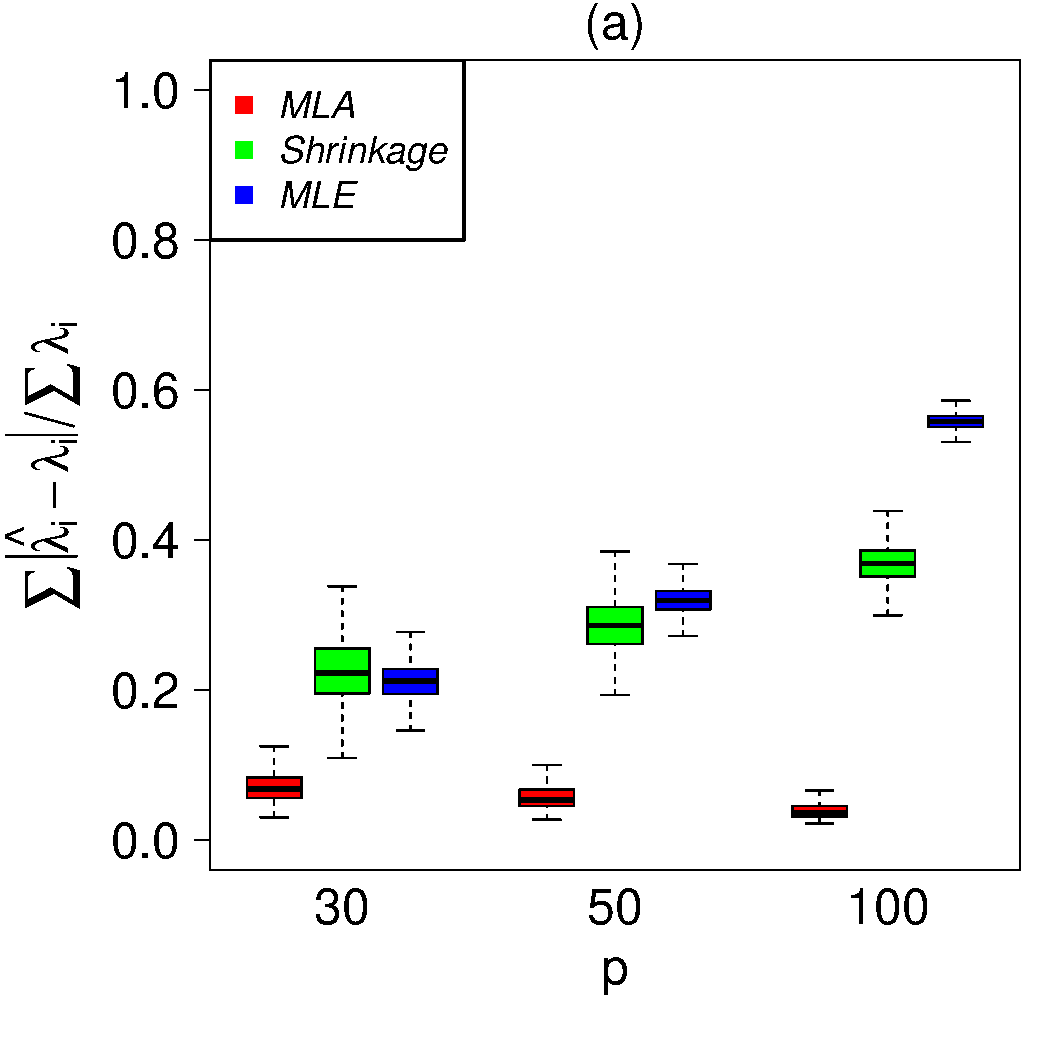
\includegraphics[scale=0.33]{FIG4_2a.pdf}
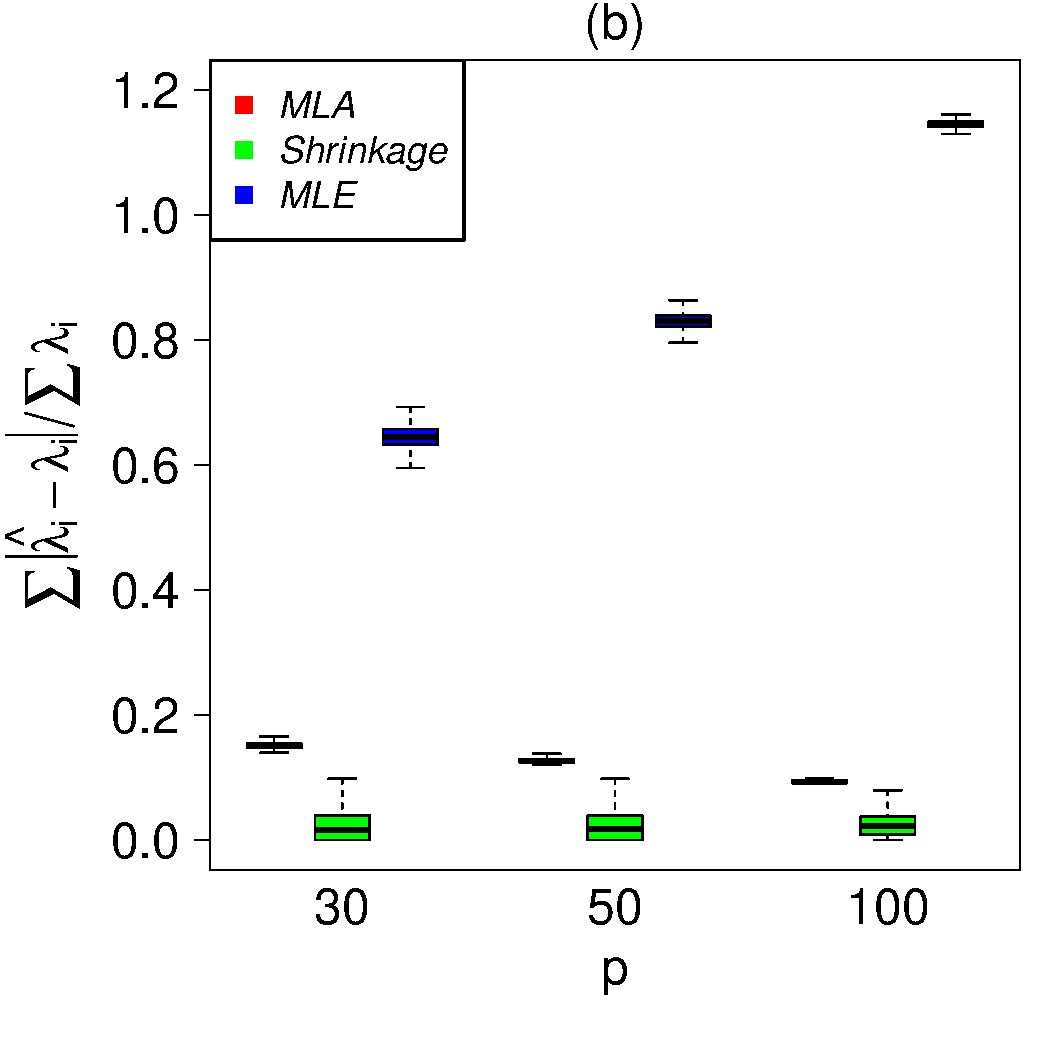
\includegraphics[scale=0.33]{FIG4_2b.pdf}
\end{array}$
\end{center}
\begin{center}$
\begin{array}{ll}
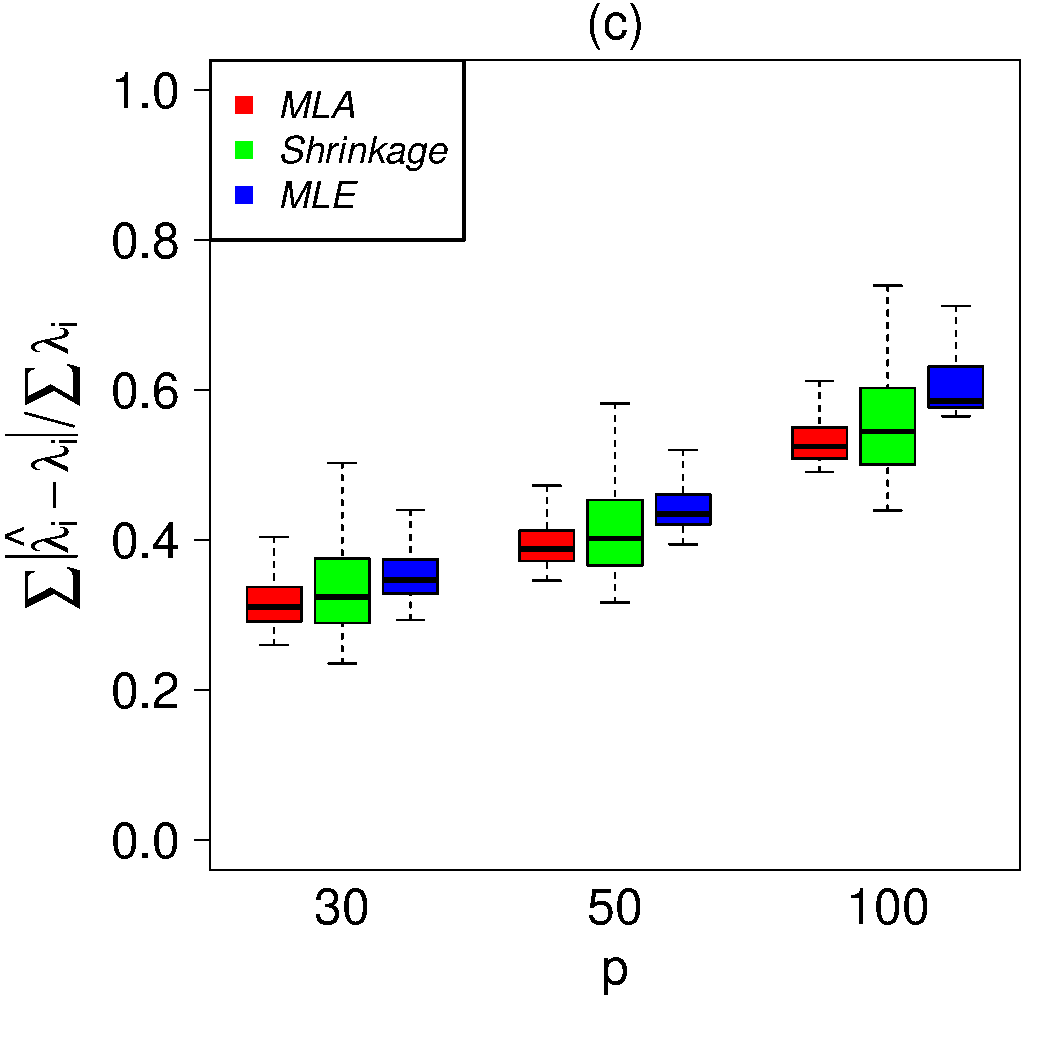
\includegraphics[scale=0.33]{FIG4_2c.pdf}
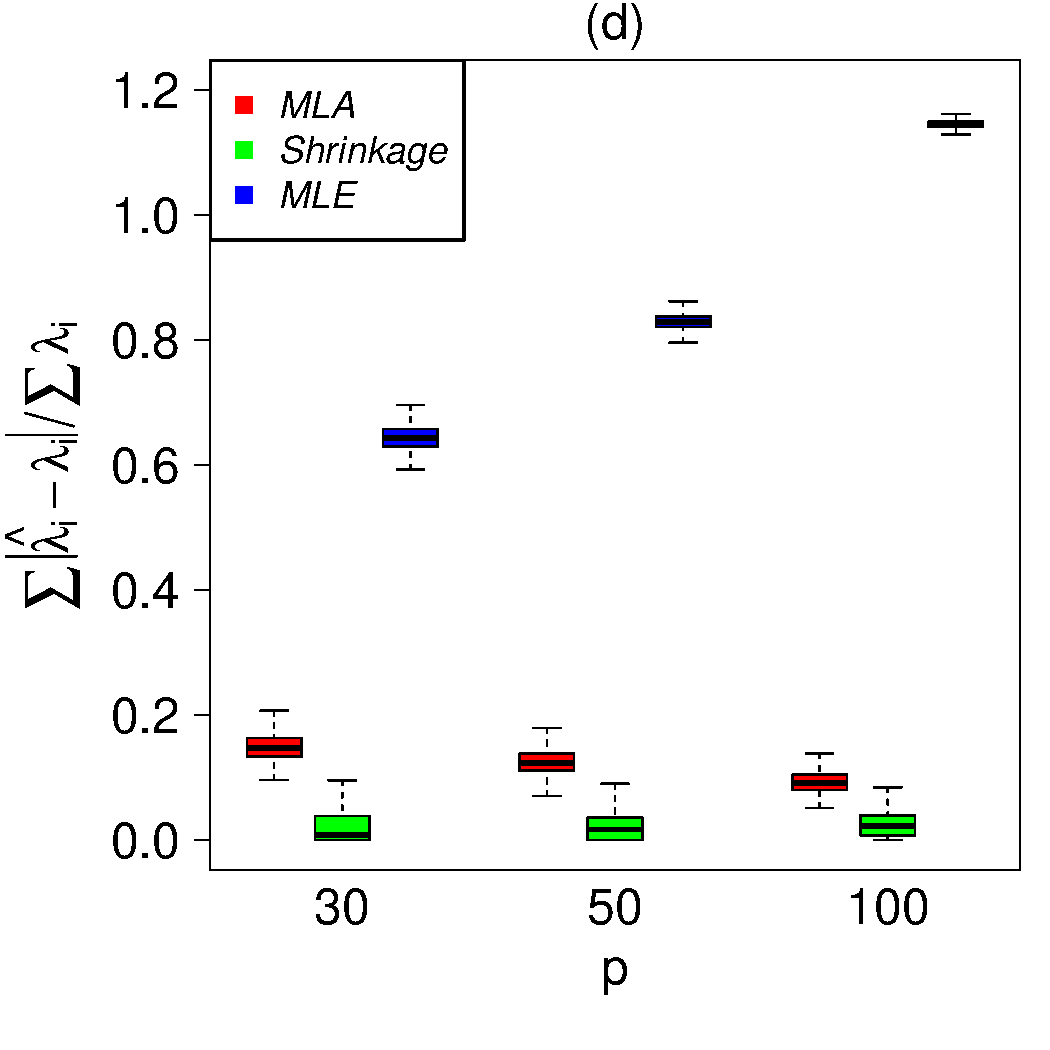
\includegraphics[scale=0.33]{FIG4_2d.pdf}
\end{array}$
\end{center}
\begin{center}$
\begin{array}{r}
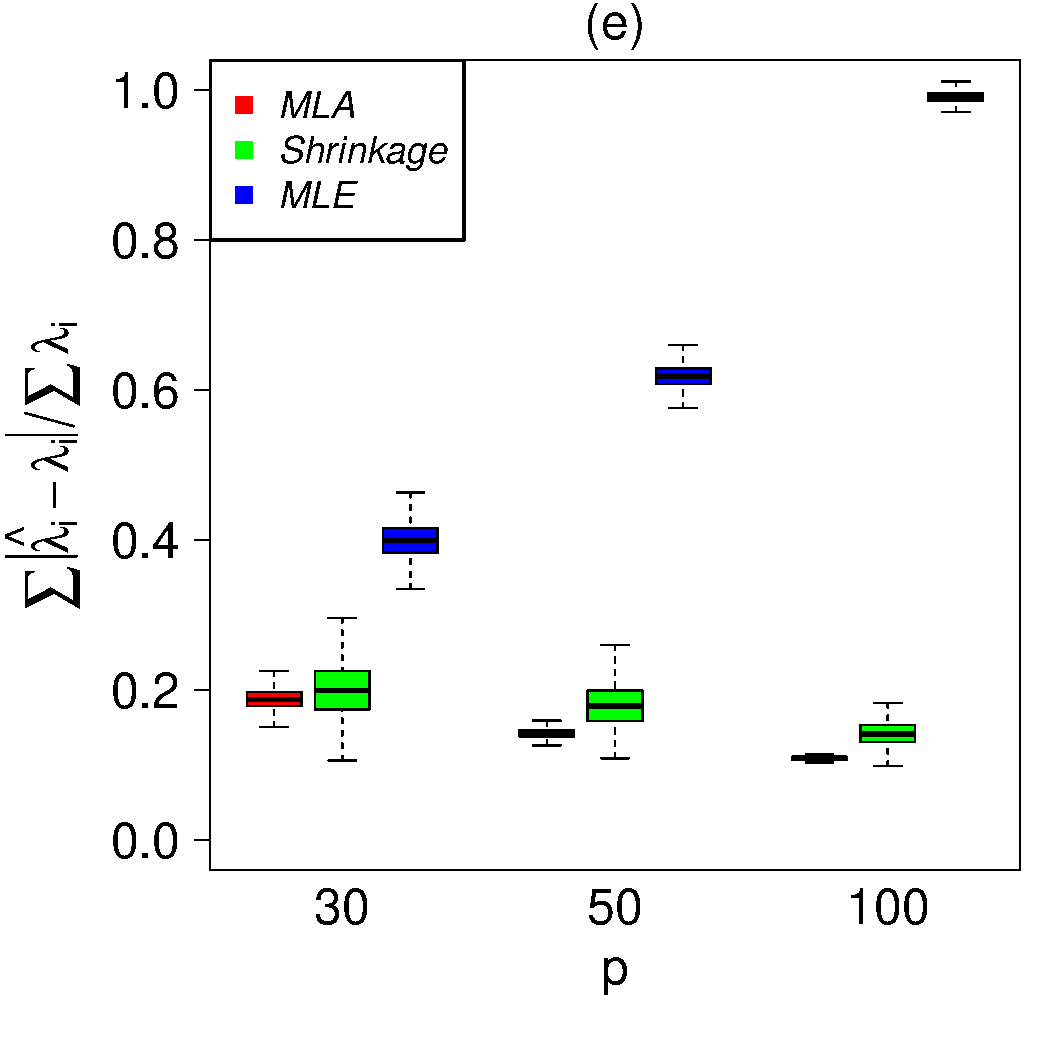
\includegraphics[scale=0.33]{FIG4_2e.pdf}
\end{array}$
\end{center}
\caption{Distribution of the sum of absolute errors in estimated eigenvalues simulated 1000 times using proposed, shrinkage and maximum likelihood methods under different choices of covariance matrices (a, b) AR(1) with $t=0.5$ and identity as true covariance matrix for all three methods and AR(1) as a target for the proposed method (c, d) exchangeable with $t=0.5$ and identity as true covariance matrix for all three methods and exchangeable as a target for the proposed method (e) random covariance structure with 30\% off-diagonal entries as non-zero and identity matrix as a target. The data are generated from multivariate normal distribution with $n=50$ and $p=\lbrace 30,50,100\rbrace$.}
\label{Fig1}
\end{figure}

%\begin{figure}[h]
%\centering
%\begin{subfigure}[t]{.4\textwidth}
%\centering
%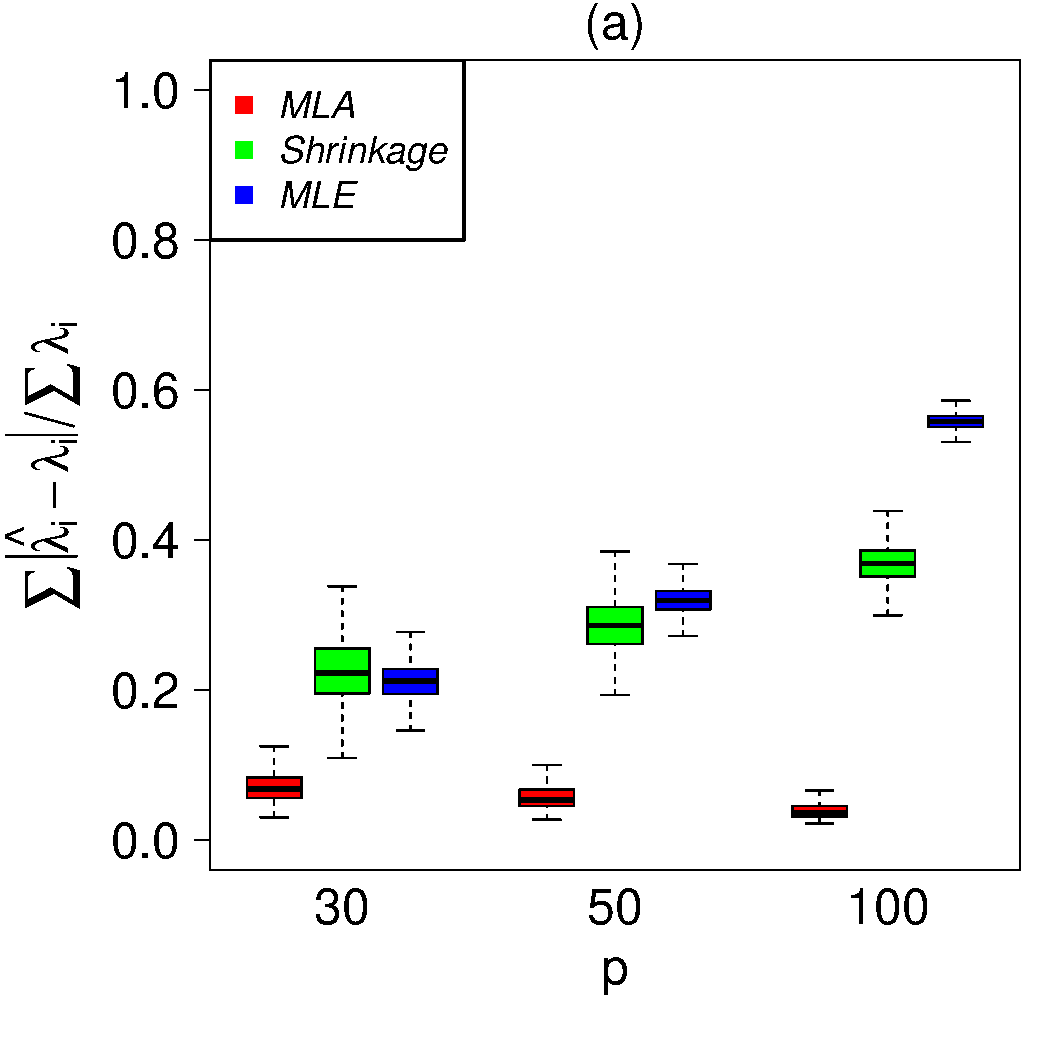
\includegraphics[width=\linewidth]{FIG4_2a.pdf}
%\end{subfigure}
%\begin{subfigure}[t]{.4\textwidth}
%\centering
%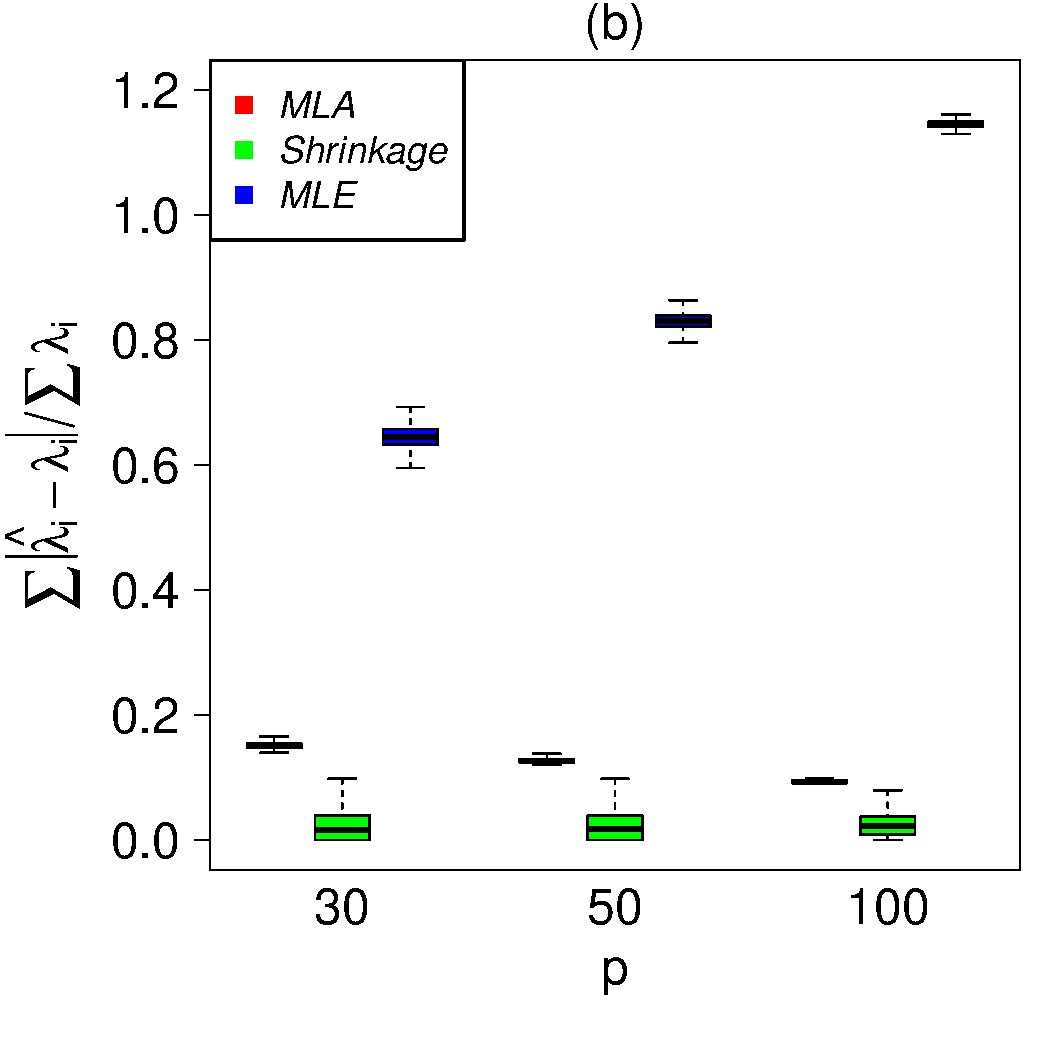
\includegraphics[width=\linewidth]{FIG4_2b.pdf}
%\end{subfigure}
%\medskip
%\begin{subfigure}[t]{.4\textwidth}
%\centering
%\vspace{0pt}
%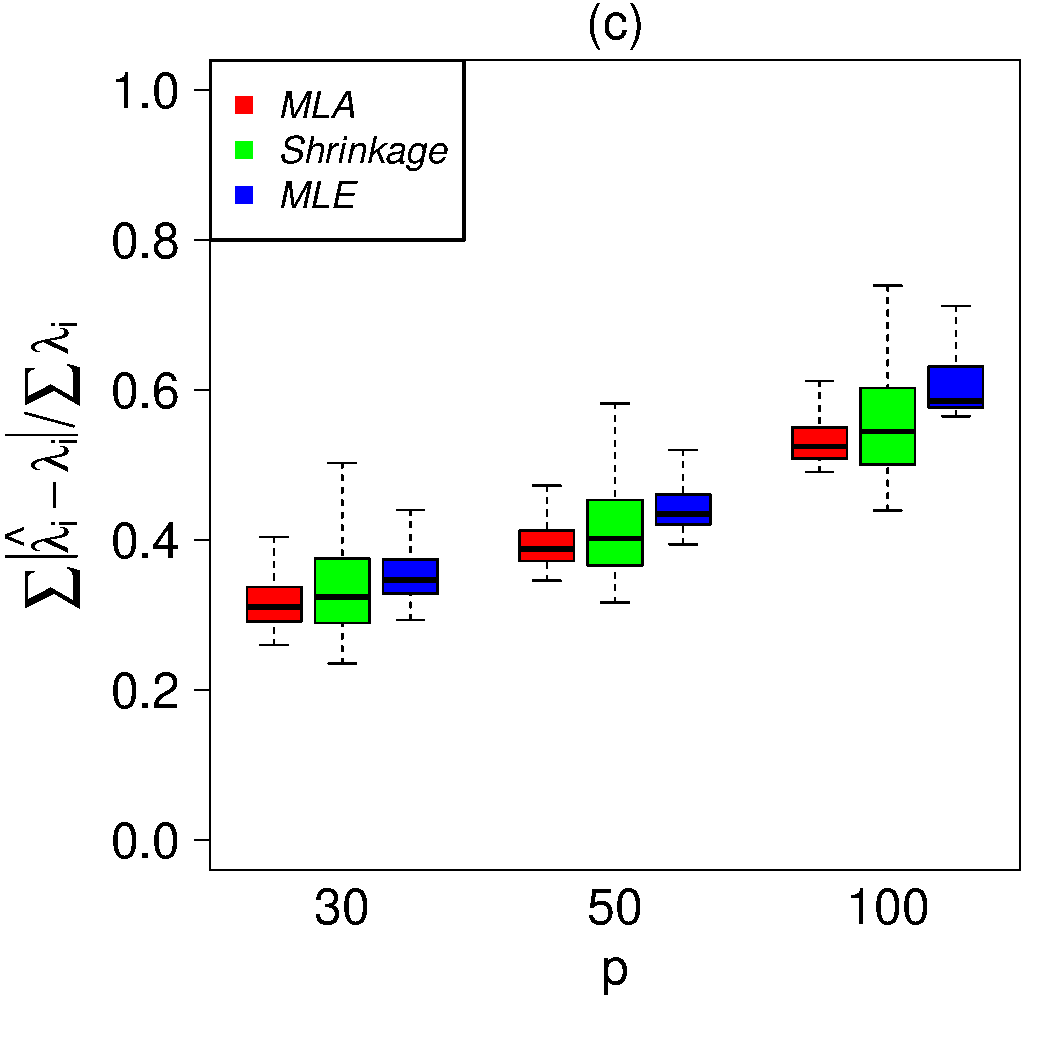
\includegraphics[width=\linewidth]{FIG4_2c.pdf}
%\end{subfigure}
%\begin{subfigure}[t]{.4\textwidth}
%\centering
%\vspace{0pt}
%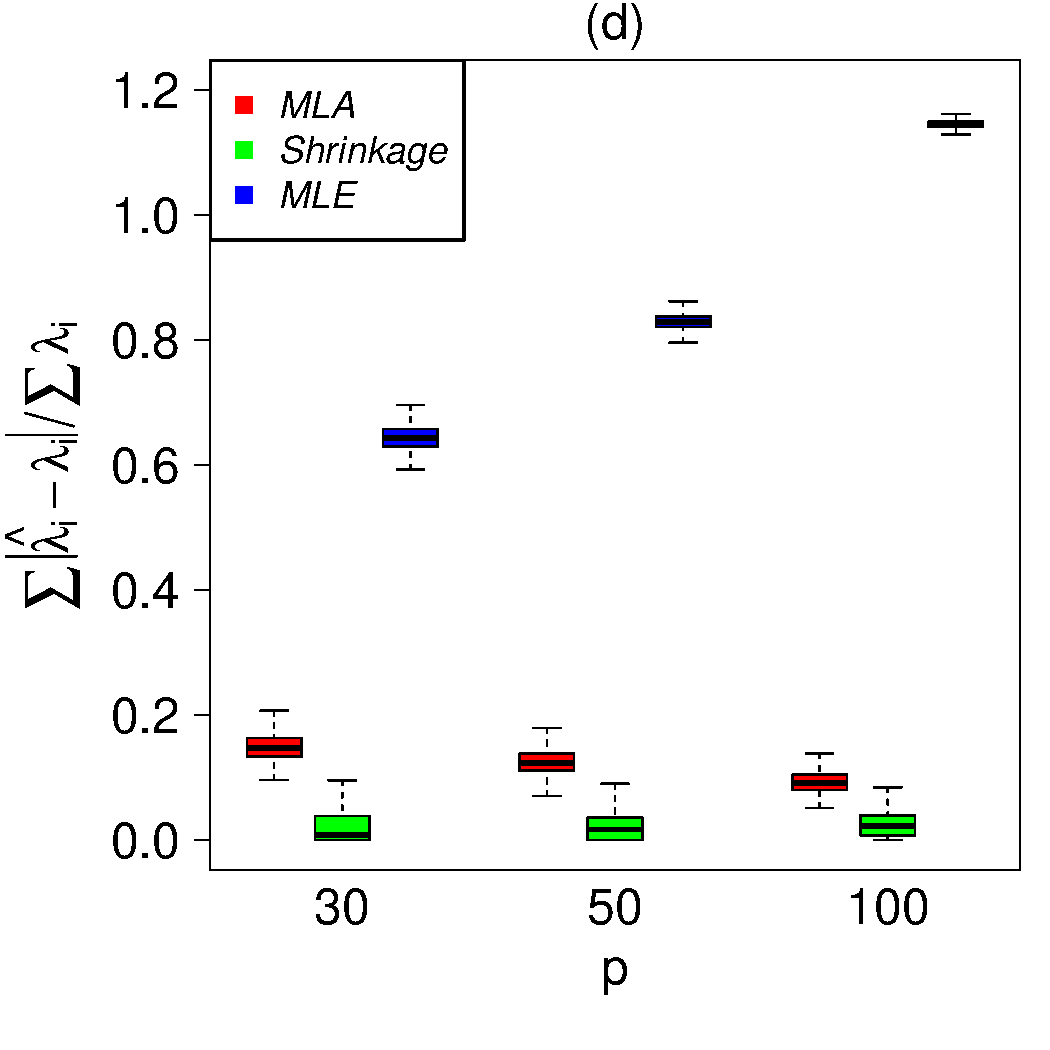
\includegraphics[width=\linewidth]{FIG4_2d.pdf}
%\end{subfigure}
%\begin{subfigure}[t]{.4\textwidth}
%\centering
%\vspace{0pt}
%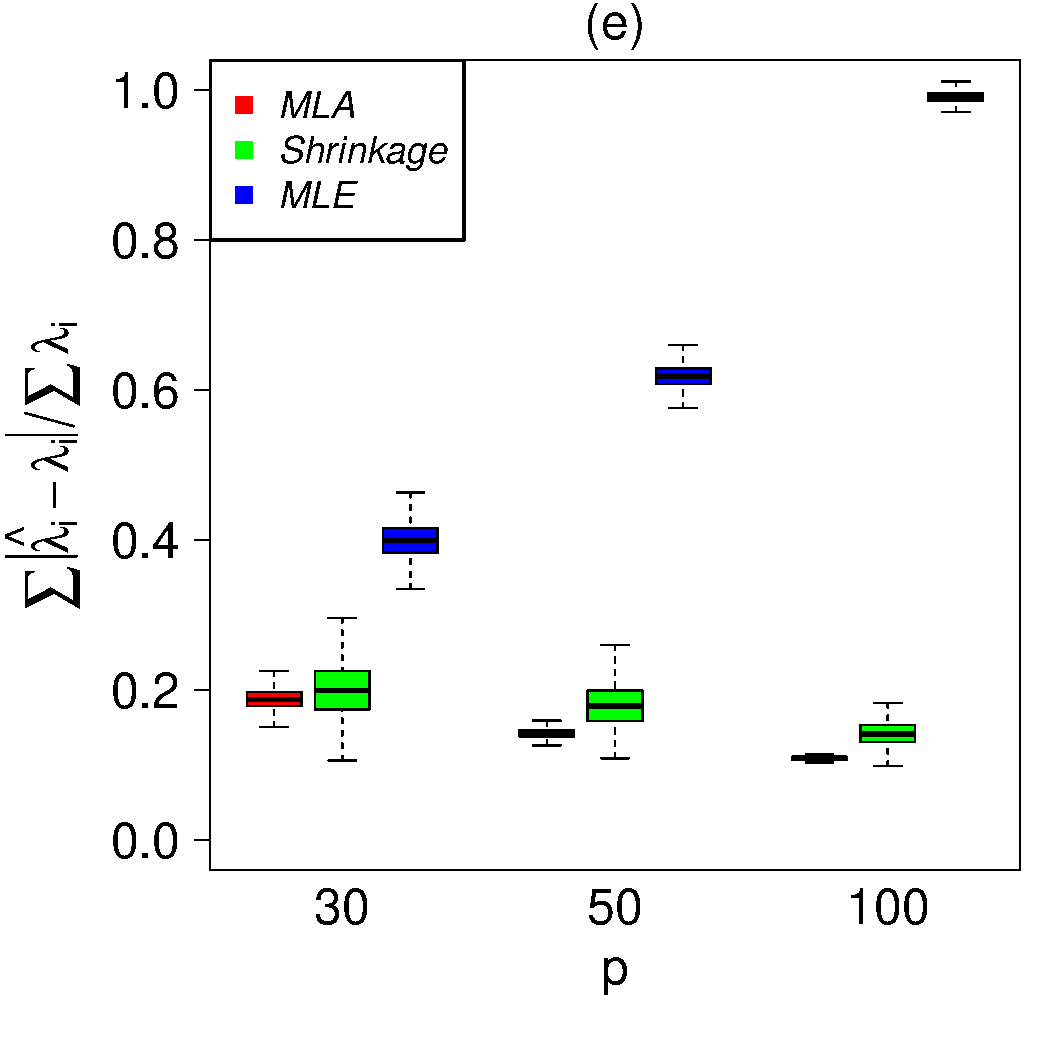
\includegraphics[width=\linewidth]{FIG4_2e.pdf}
%\end{subfigure}
%\caption{Distribution of the sum of absolute errors in estimated eigenvalues simulated 1000 times using proposed, shrinkage and maximum likelihood methods under different choices of covariance matrices and targets for the proposed method arranged in Table \ref{Tab1}. For random covariance structure we took 30\% of the off-diagonal entries as non-zero. The data are generated from multivariate normal distribution with $n=50$ and $p=\lbrace 30,50,100\rbrace$.}
%\label{Fig1}
%\end{figure}
%(a, b) AR(1) covariance structure, (c, d) exchangeable covariance structure, (c) random covariance matrix with $30\%$ proportion on non-zero off-diagonal elements for sample of size $n=50$ from a multivariate normal distribution with $p=\lbrace 30,50,100\rbrace$. These results are simulated 1000 times.
%We use the same covariance structures with parameter values to simulate the data from multivariate normal distribution and with the same targets as was used in the first experiment.
%If the true covariance matrix is AR(1) or exchangeable covariance structure, in that instances we shrink the sample covariance matrix towards two targets: a correct target that is, respectively, AR(1) and exchangeable and incorrect target: identity matrix

For the second type of experiments, we show the results for increasing value of $n= 10,20,30,40,50,60,70,90,120,200$ while keeping $p=10$. In this case we show the asymptotic performance of the competing methods. We use all three aforementioned covariance structures and simulate the data from multivariate normal distribution as we did in the previous case. For this case, we also consider $t=0.5$ for both AR(1) and exchangeable covariance structures and for random covariance structure we take 30\% non-zero off-diagonal elements. When the true covariance matrices are AR(1) and exchangeable we shrink the sample covariance matrix, respectively, towards AR(1) and exchangeable targets, which are correct targets for AR(1) and exchangeable covariance structures. For identity as a true covariance matrix we also use both AR(1) and exchangeable targets to shrink the sample covariance matrix towards them, which is incorrect. In case of random covariance structure we shrink the sample covariance matrix towards the identity matrix (commonly used target to regularized sample covariance matrix whenever $p \gg n$). We then calculate sum of element-wise squared errors (denoted by MSE in the rest of the thesis) of the estimated covariance matrices given by $ \norm{\boldsymbol{\hat{\Sigma}} - \boldsymbol{\Sigma}}_{F}^{2}$, 
%\begin{equation*}
%L(\boldsymbol{\hat{\Sigma}}, \boldsymbol{\Sigma}) = \norm{\boldsymbol{\hat{\Sigma}} - \boldsymbol{\Sigma}}_{F}^{2},
%\label{equ2}
%\end{equation*}
where $\norm{.}^{2}_{F}$ denotes the sum of element-wise squared errors also known as squared Frobenius norm. Figure \ref{Fig2} shows the MSE of three different methods averaged over 1000 simulations.
\section*{Results:}
From the simulation results, it is clear that the best estimator in terms of MSE is the one obtained from the proposed method when the target is correctly specified in case of AR(1) and exchangeable covariance structures. However, as can be expected, the performance of the other methods become similar when the sample size is very large. However, the proposed method perform slightly poor than the shrinkage method when the target is incorrectly specified as AR(1) or exchangeable while the true covariance matrix is identity matrix. For the random covariance structure the proposed method has minimum mean squared error than the shrinkage method when $n \approx p$, but as $n$ increases its mean squared error is also increases indicating that the proposed estimator is asymptotically more biased (the case when the maximum likelihood estimate is valid). 

\begin{figure}[H]
\begin{center}$
\begin{array}{ll}
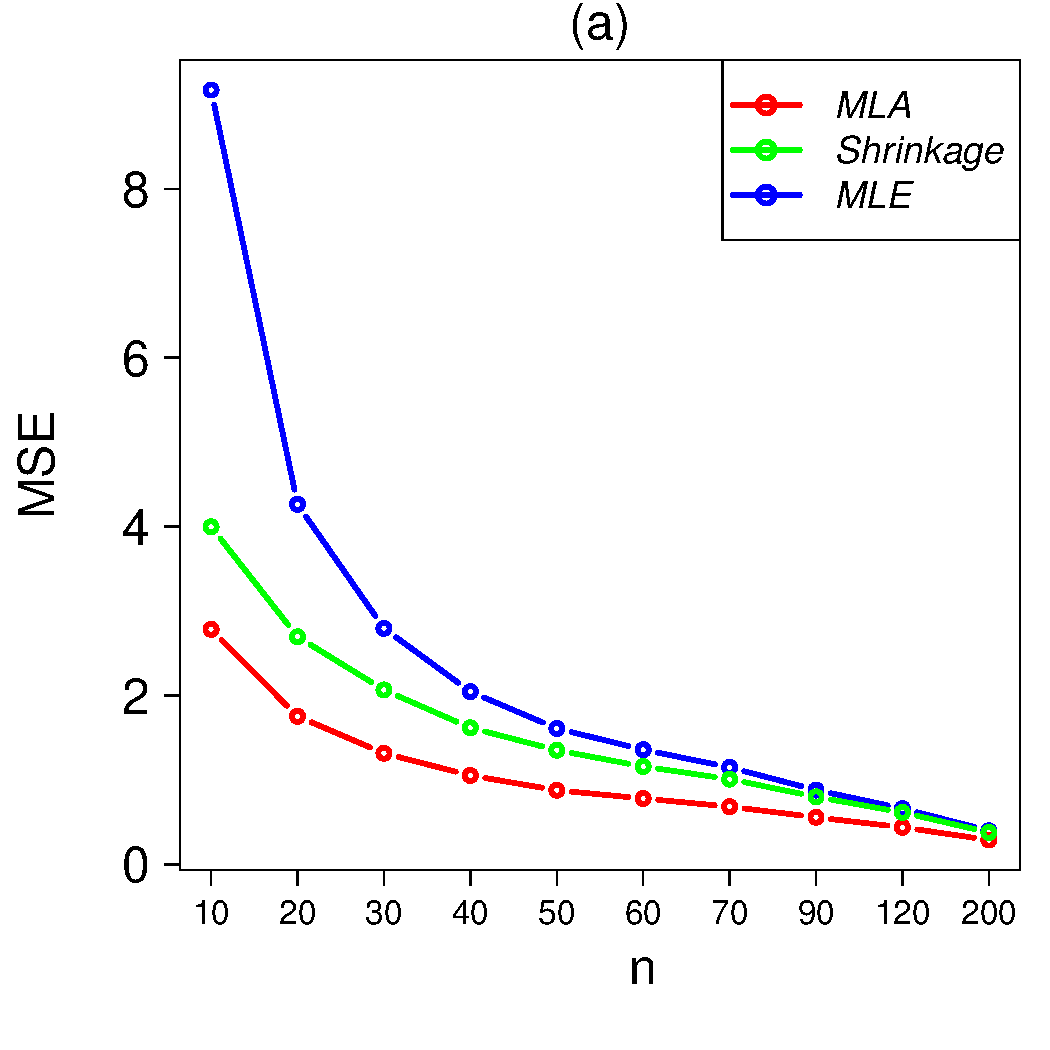
\includegraphics[scale=0.33]{FIG4_4a.pdf}
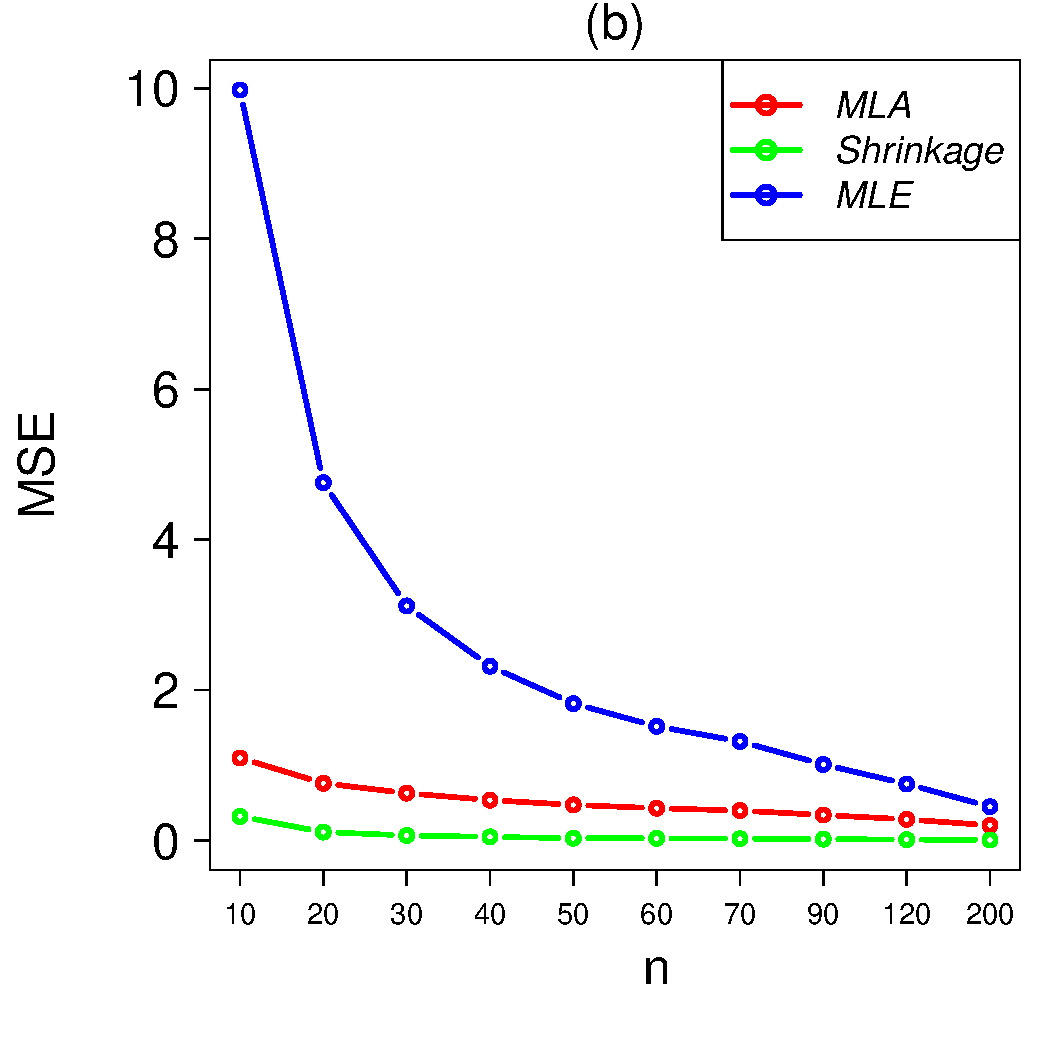
\includegraphics[scale=0.33]{FIG4_4b.pdf}
\end{array}$
\end{center}
\begin{center}$
\begin{array}{ll}
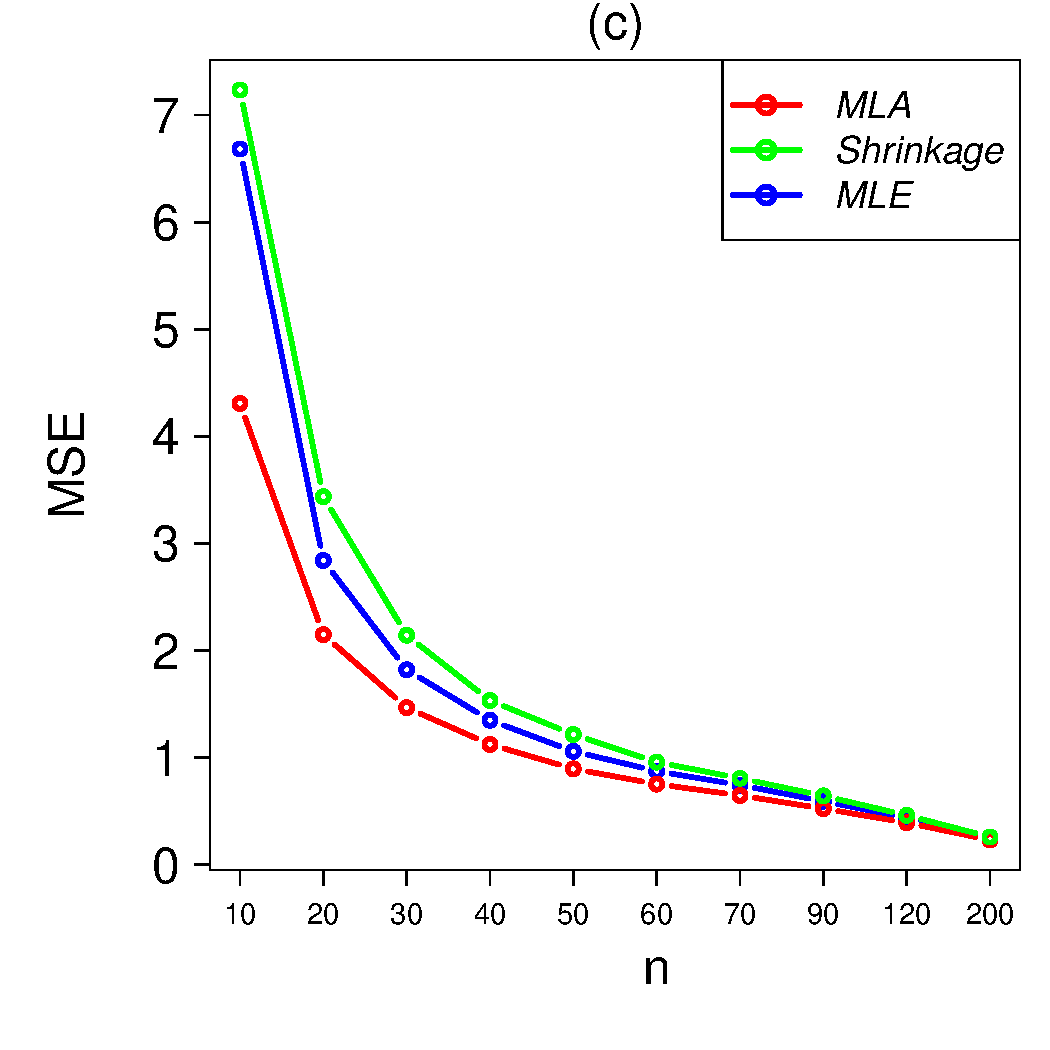
\includegraphics[scale=0.33]{FIG4_4c.pdf}
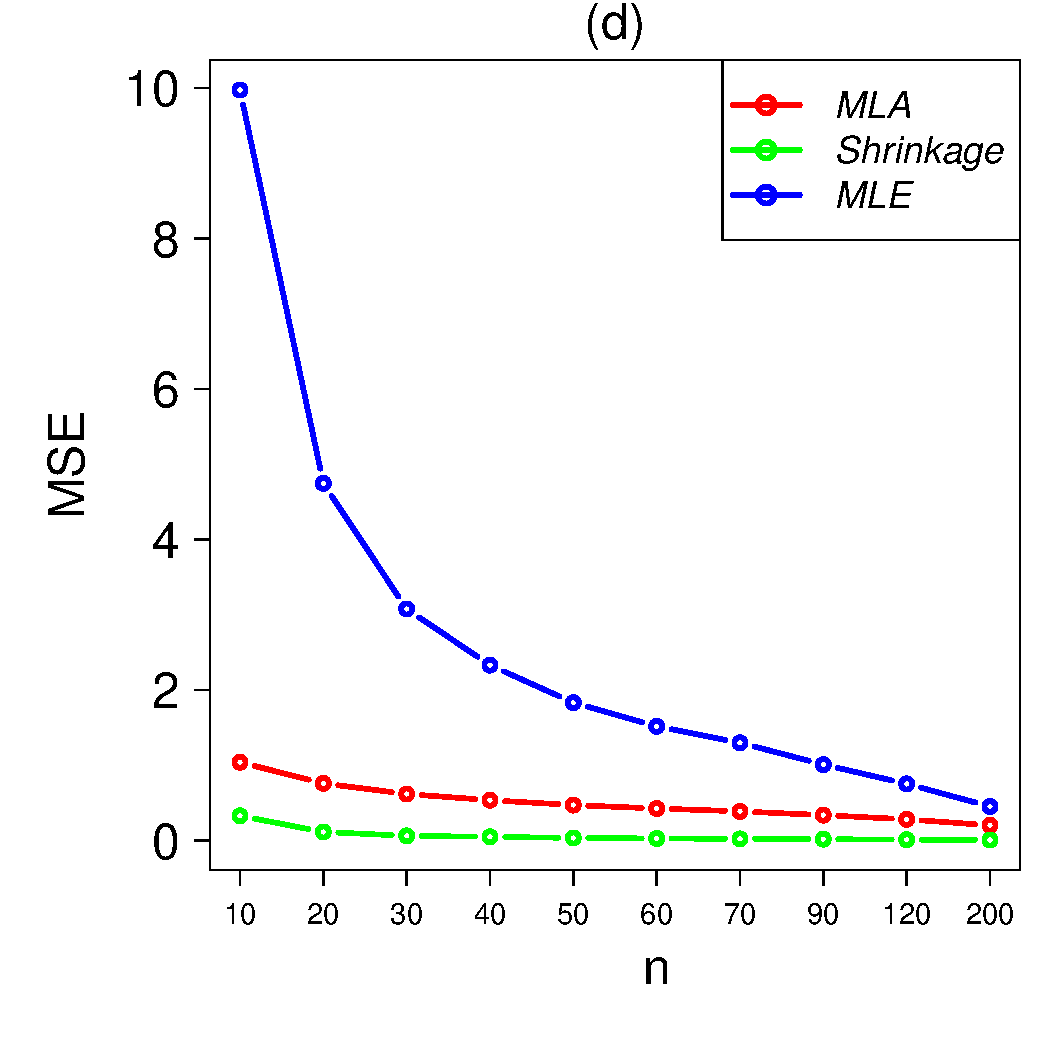
\includegraphics[scale=0.33]{FIG4_4d.pdf}
\end{array}$
\end{center}
\begin{center}$
\begin{array}{r}
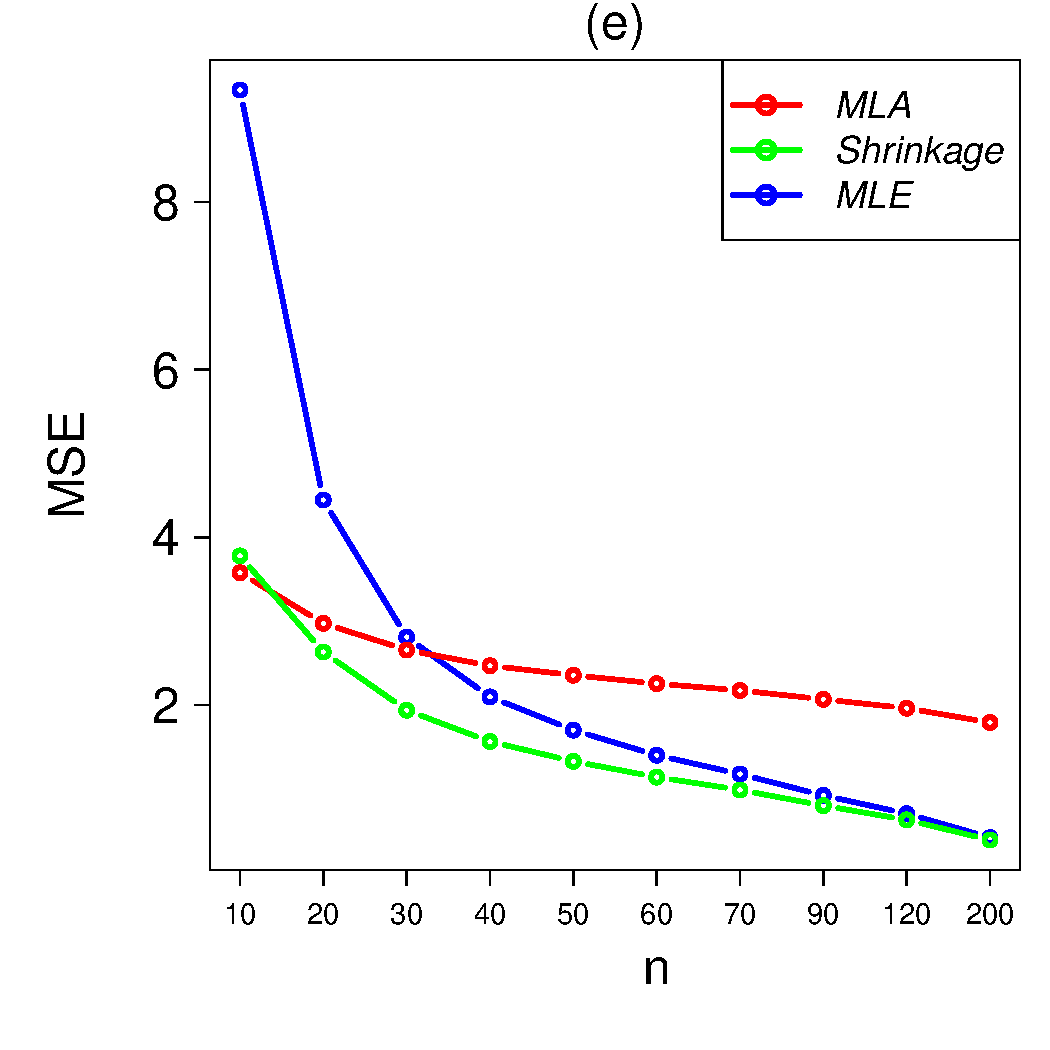
\includegraphics[scale=0.33]{FIG4_4e.pdf}
\end{array}$
\end{center}
\caption{Comparison of MSE averaged over 1000 simulations of the estimated covariance matrices. The data are drawn from multivariate normal distribution with sample size $n=\lbrace10, 20,30,40,50,60,70,90,120,200\rbrace$ and $p=10$ under different choices of covariance matrices (a, b) AR(1) with $t=0.5$ and identity as true covariance matrix for all three methods and AR(1) as a target for the proposed method (c, d) exchangeable with $t=0.5$ and identity as true covariance matrix for all three methods and exchangeable as a target for the proposed method (e) random covariance structure with 30\% off-diagonal entries as non-zero and identity matrix as a target.}
\label{Fig2}
\end{figure}

 
%\begin{figure}[h]
%\centering
%\begin{subfigure}[t]{.4\textwidth}
%\centering
%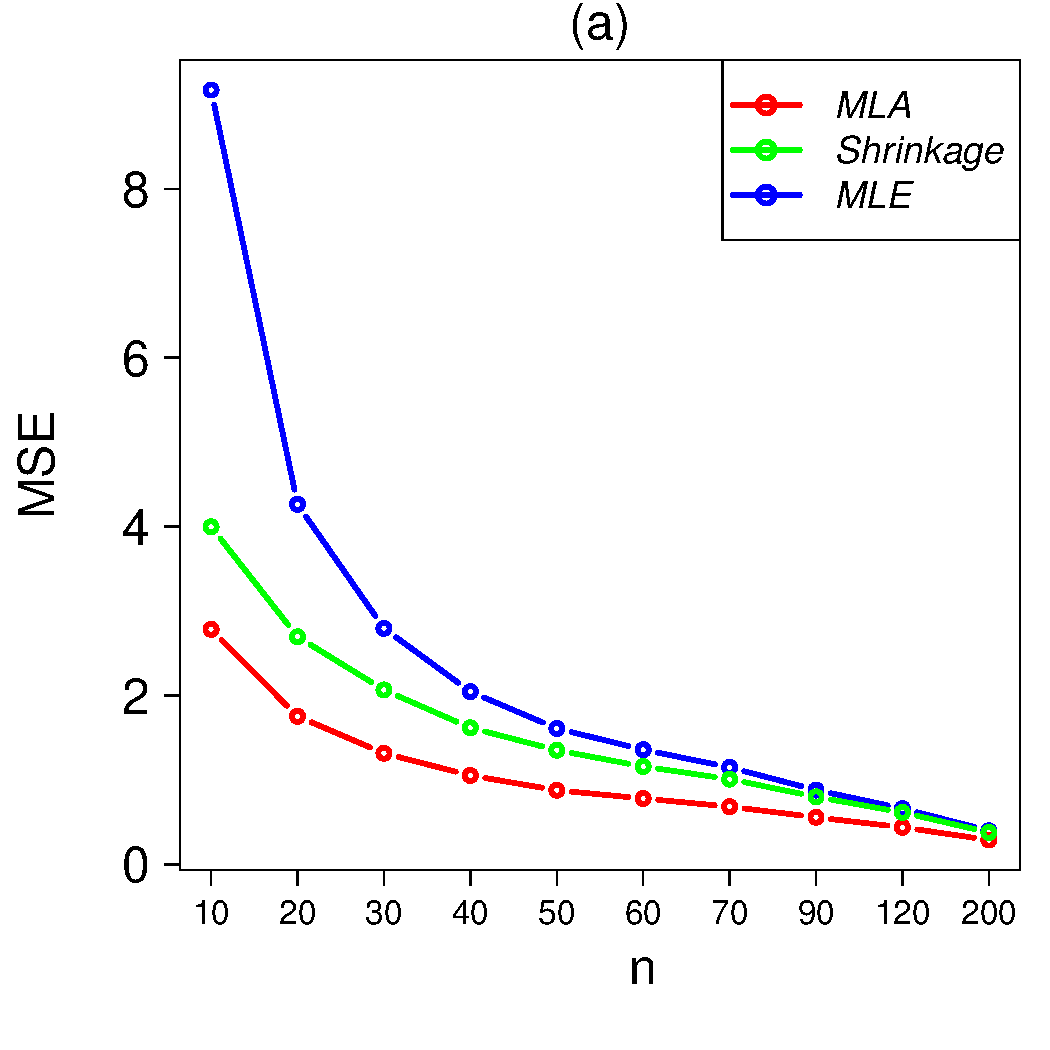
\includegraphics[width=\linewidth]{FIG4_4a.pdf}
%\end{subfigure}
%\begin{subfigure}[t]{.4\textwidth}
%\centering
%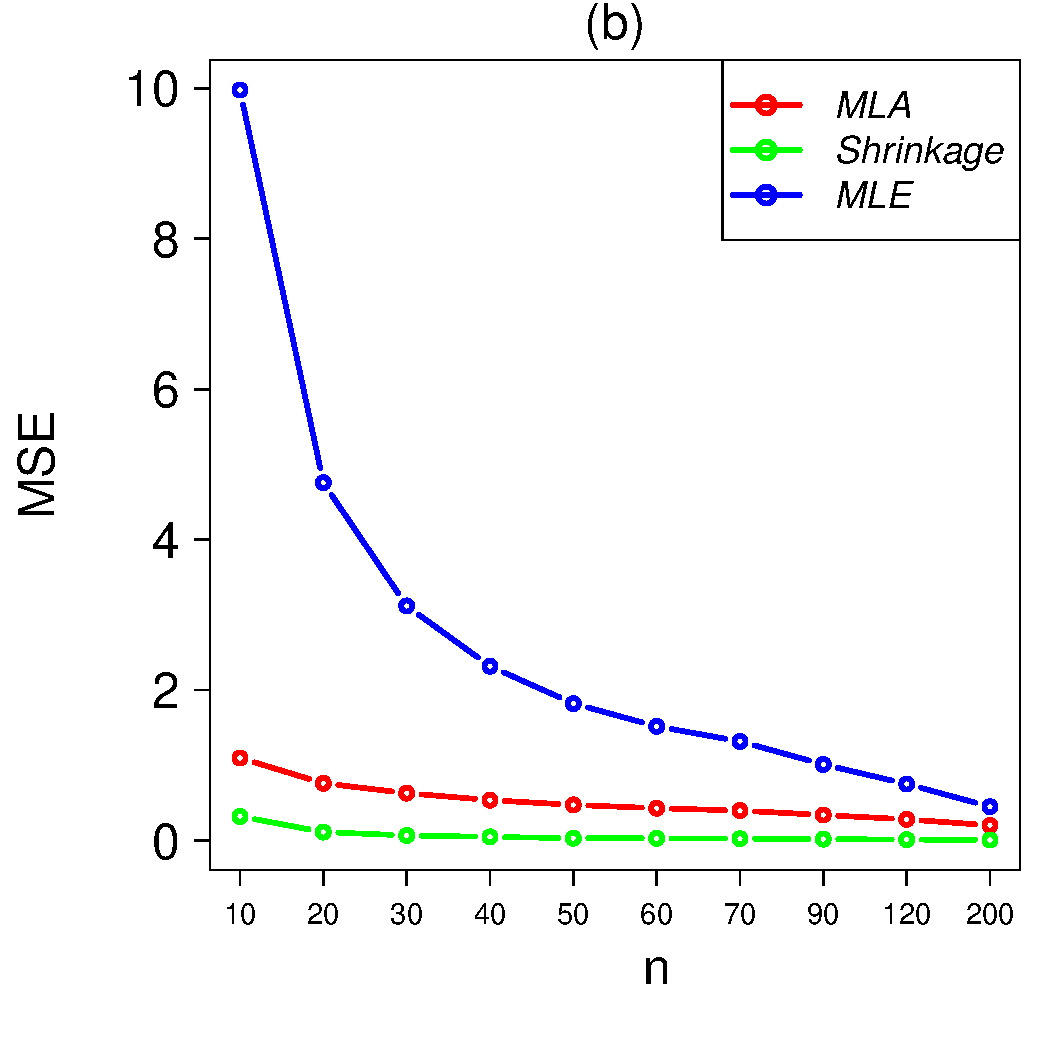
\includegraphics[width=\linewidth]{FIG4_4b.pdf}
%\end{subfigure}
%\medskip
%\begin{subfigure}[t]{.4\textwidth}
%\centering
%\vspace{0pt}
%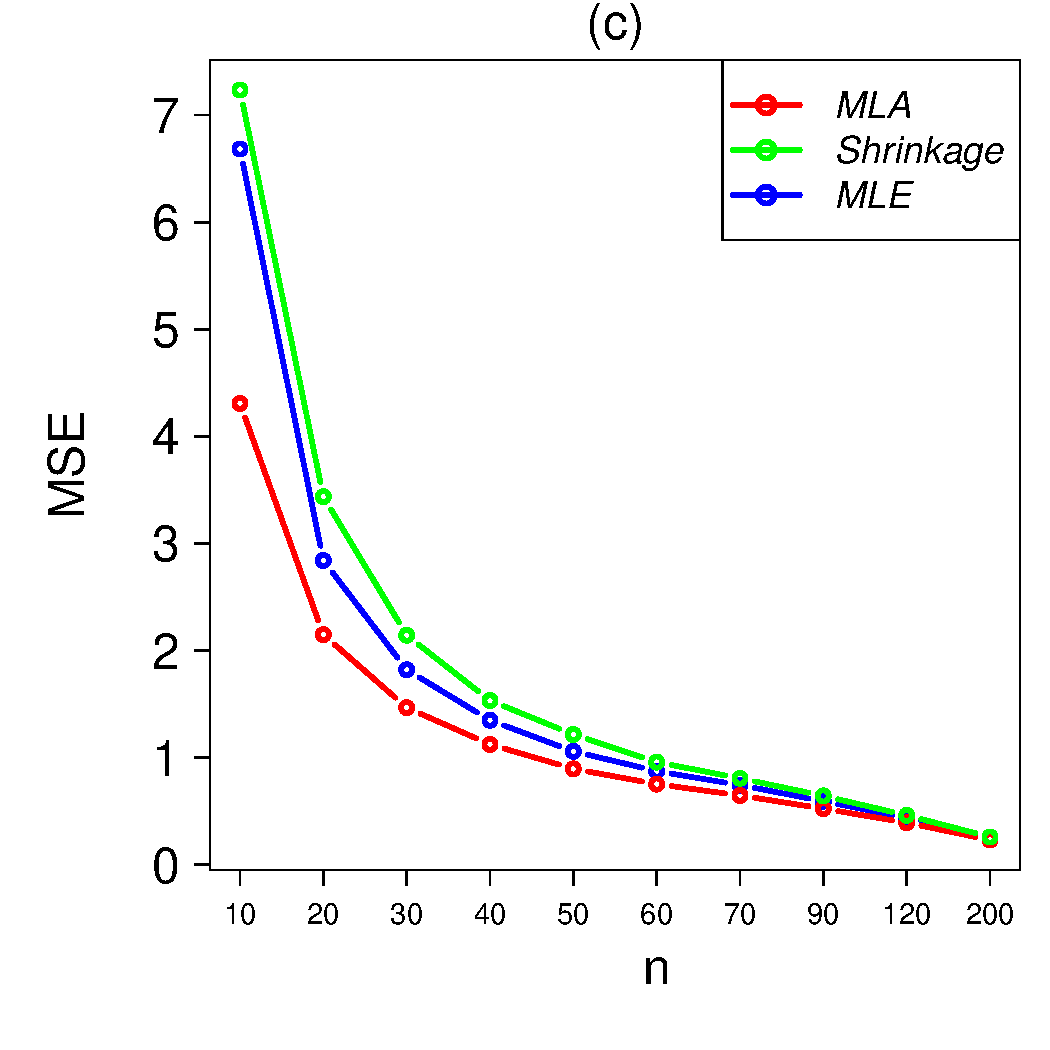
\includegraphics[width=\linewidth]{FIG4_4c.pdf}
%\end{subfigure}
%\begin{subfigure}[t]{.4\textwidth}
%\centering
%\vspace{0pt}
%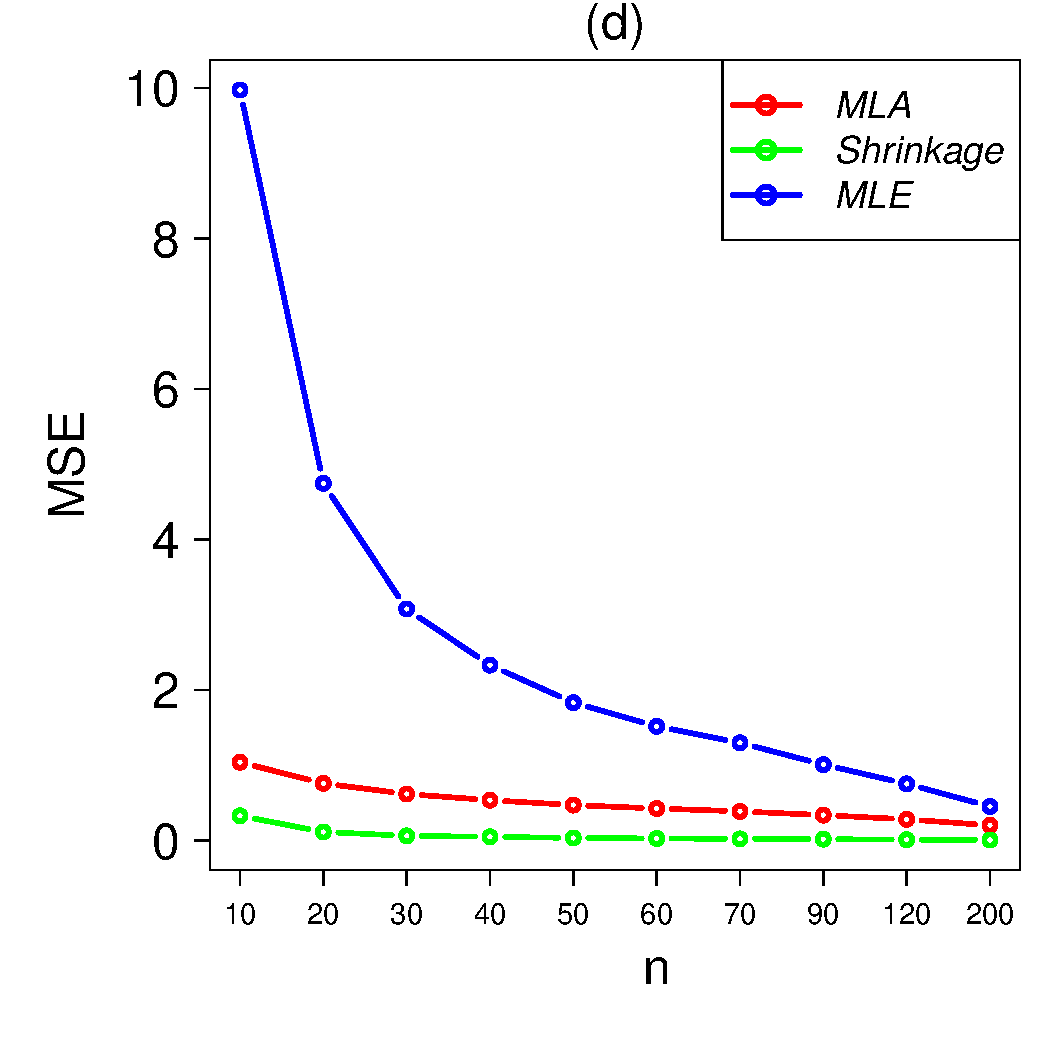
\includegraphics[width=\linewidth]{FIG4_4d.pdf}
%\end{subfigure}
%\begin{subfigure}[t]{.4\textwidth}
%\centering
%\vspace{0pt}
%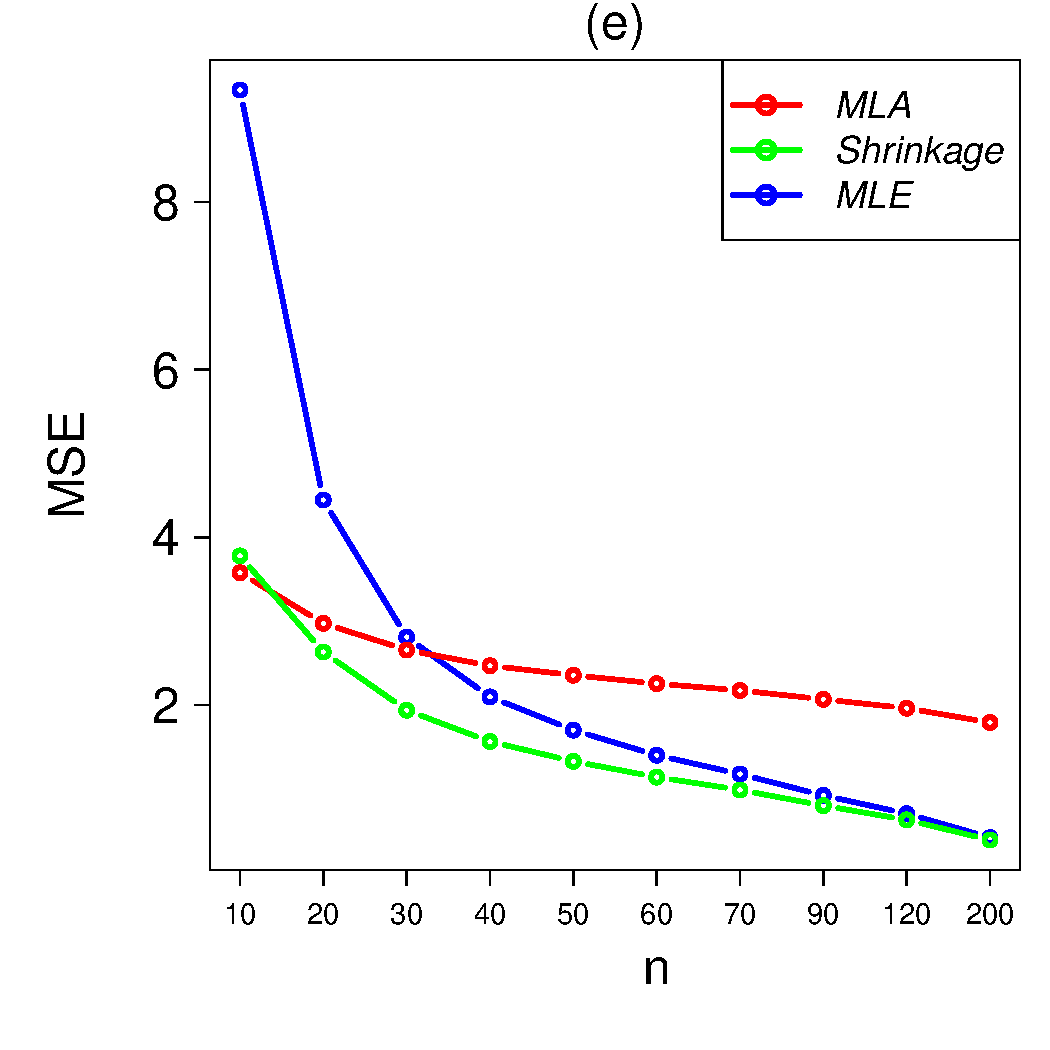
\includegraphics[width=\linewidth]{FIG4_4e.pdf}
%\end{subfigure}
%\caption{Comparison of MSE averaged over 1000 simulations of the estimated covariance matrices. The data are drawn from multivariate normal distribution with sample size $n=\lbrace10, 20,30,40,50,60,70,90,120,200\rbrace$ and $p=10$. Three different structures of the covariance matrices and targets only for the proposed method arranged in Table \ref{Tab1} are used. For random covariance structure we took 30\% off-diagonal entries as being non-zero.}
%\label{Fig2}
%\end{figure}
%, i.e, (a, b) AR(1) covariance structure with targets AR(1) and identity matrix and $t=0.5$, (c, d) exchangeable covariance structure with targets exchangeable and identity matrix and $t=0.5$, (c)
%In third experiment, we plot the eigenvalues of the estimated covariance matrices of proposed method, shrinkage method of \cite{schafer2005shrinkage}, maximum likelihood method and eigenvalues of the true covariance matrix. We set $n=30$ and $p=50$ and use the same covariance structures to simulate the data from multivariate normal distribution and targets for different covariance structures as was used in the above two experiments, the only difference in this case is that for exchangeable covariance structure we consider $t=0.3$

In the previous case, we demonstrated the estimation error in eigenvalues. Here we visually compare the estimated eigenvalues with the true eigenvalue. Although we have conducted a range of simulation experiments, we show the results for $n=30$ and $p=50$ and generate the data from multivariate normal distribution using all three covariance structures mentioned above. For AR(1) and exchangeable covariance structures we consider $t=0.5$ and $t=0.3$, respectively. For random covariance structure we take 30\% of the off-diagonal elements as being non-zero. Furthermore, when the true covariance matrices are AR(1) and exchangeable we shrink the sample covariance matrix, respectively, towards AR(1) and exchangeable targets, which are correct targets for AR(1) and exchangeable covariance structures. For identity as a true covariance matrix we also use both AR(1) and exchangeable targets to shrink the sample covariance matrix towards them, which are incorrect targets. However, for random covariance structure we use only identity matrix as a target. We then estimate the covariance matrix using the proposed and shrinkage methods and calculate the eigenvalues of the two competing estimators along with the eigenvalues of sample covariance and true covariance matrix (gold standard). These eigenvalues are presented in Figure \ref{Fig3} averaged over 1000 simulations for all three the estimated covariance matrices. 
\section*{Results:}
From Figure \ref{Fig3} it can be seen that the sample eigenvalues are highly inaccurate that is the large eigenvalues overestimated and the small eigenvalues are under estimated. The proposed method and shrinkage method of \cite{schafer2005shrinkage} overcome this problem. But the eigenvalues of the proposed method recover the true eigenvalues more accurately compare to the shrinkage method of \cite{schafer2005shrinkage} if the target is correctly specified in case of AR(1) and exchangeable covariance structures. When the target is incorrectly specified in that case the eigenvalues estimated using shrinkage method are slightly closer to the true eigenvalues as compare to the proposed method. For random covariance structure the eigenvalues obtained from the proposed estimator are more accurate. 

\begin{figure}[H]
\begin{center}$
\begin{array}{ll}
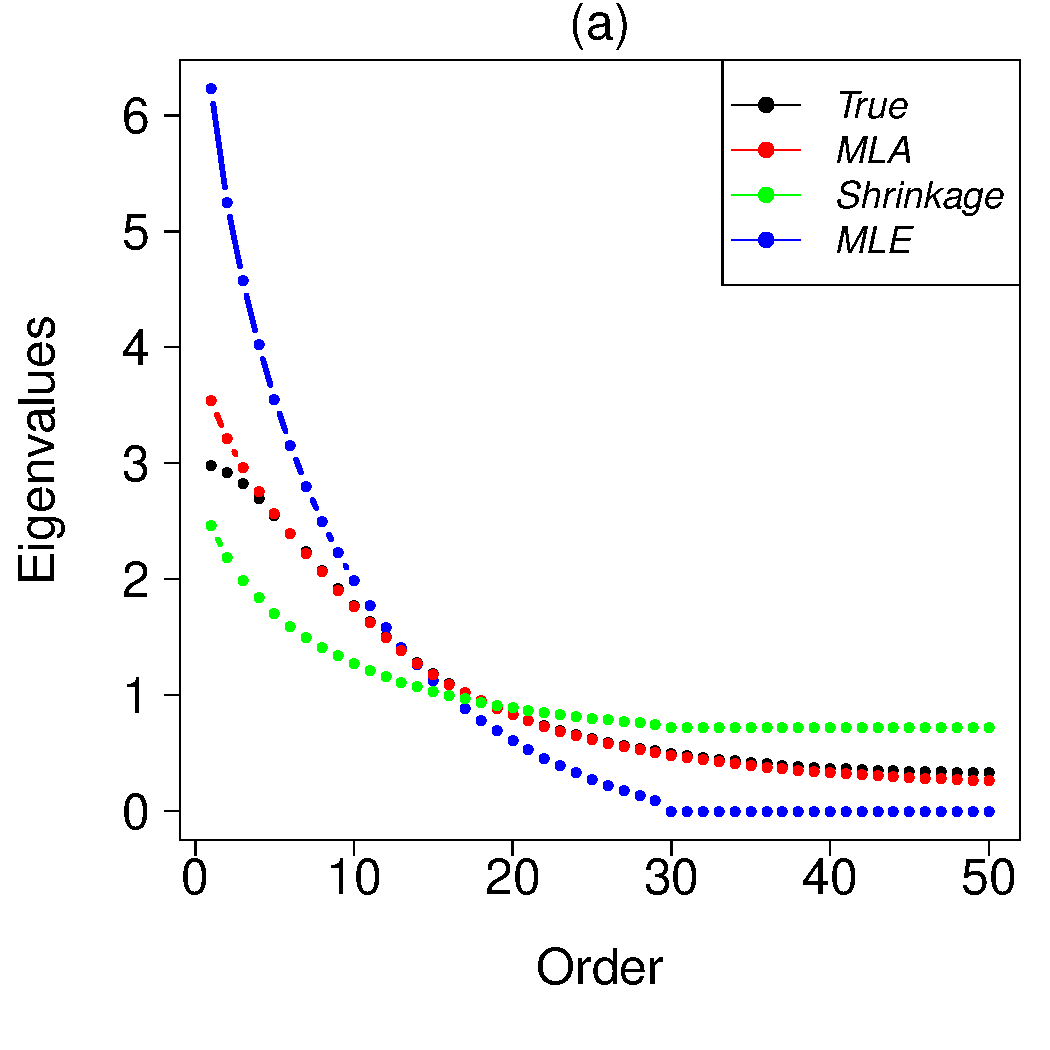
\includegraphics[scale=0.33]{FIG4_3a.pdf}
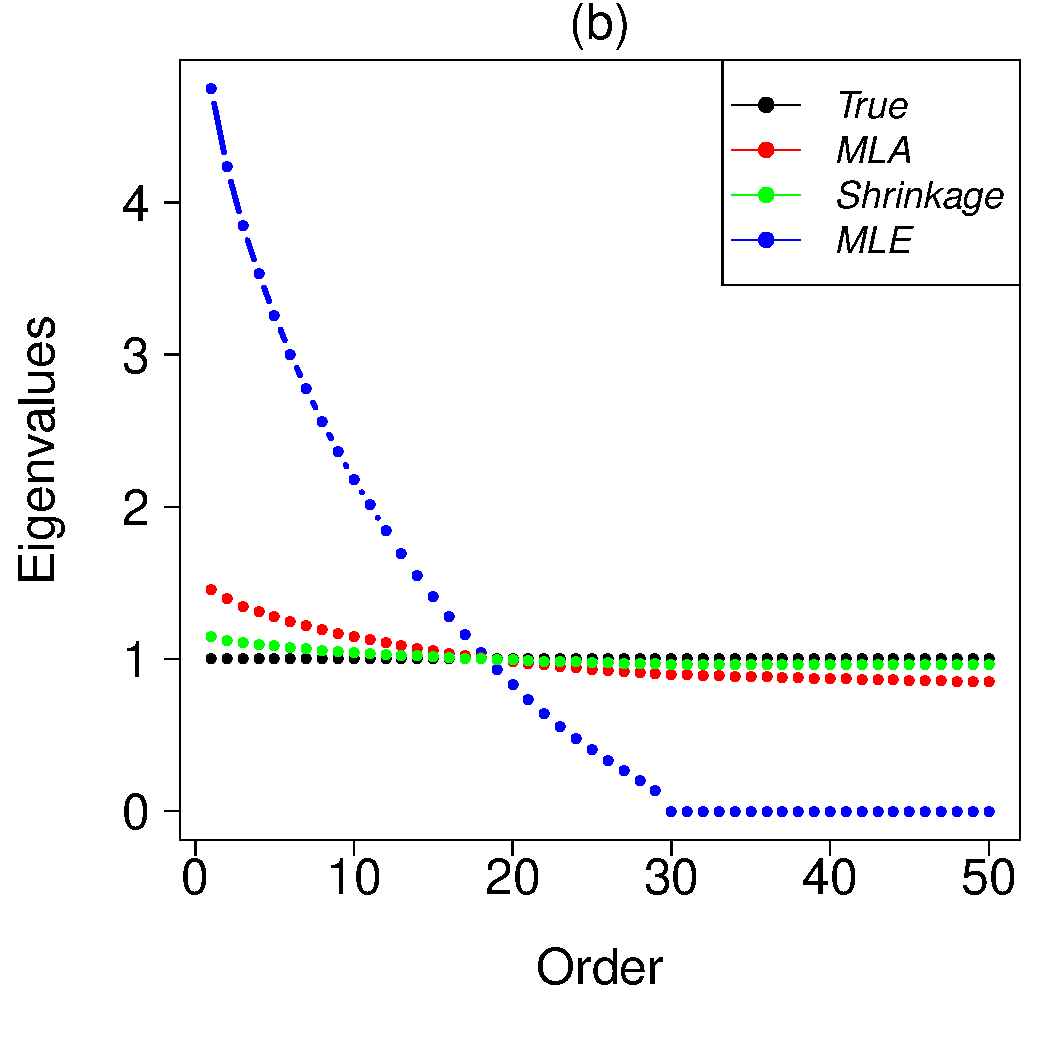
\includegraphics[scale=0.33]{FIG4_3b.pdf}
\end{array}$
\end{center}
\begin{center}$
\begin{array}{ll}
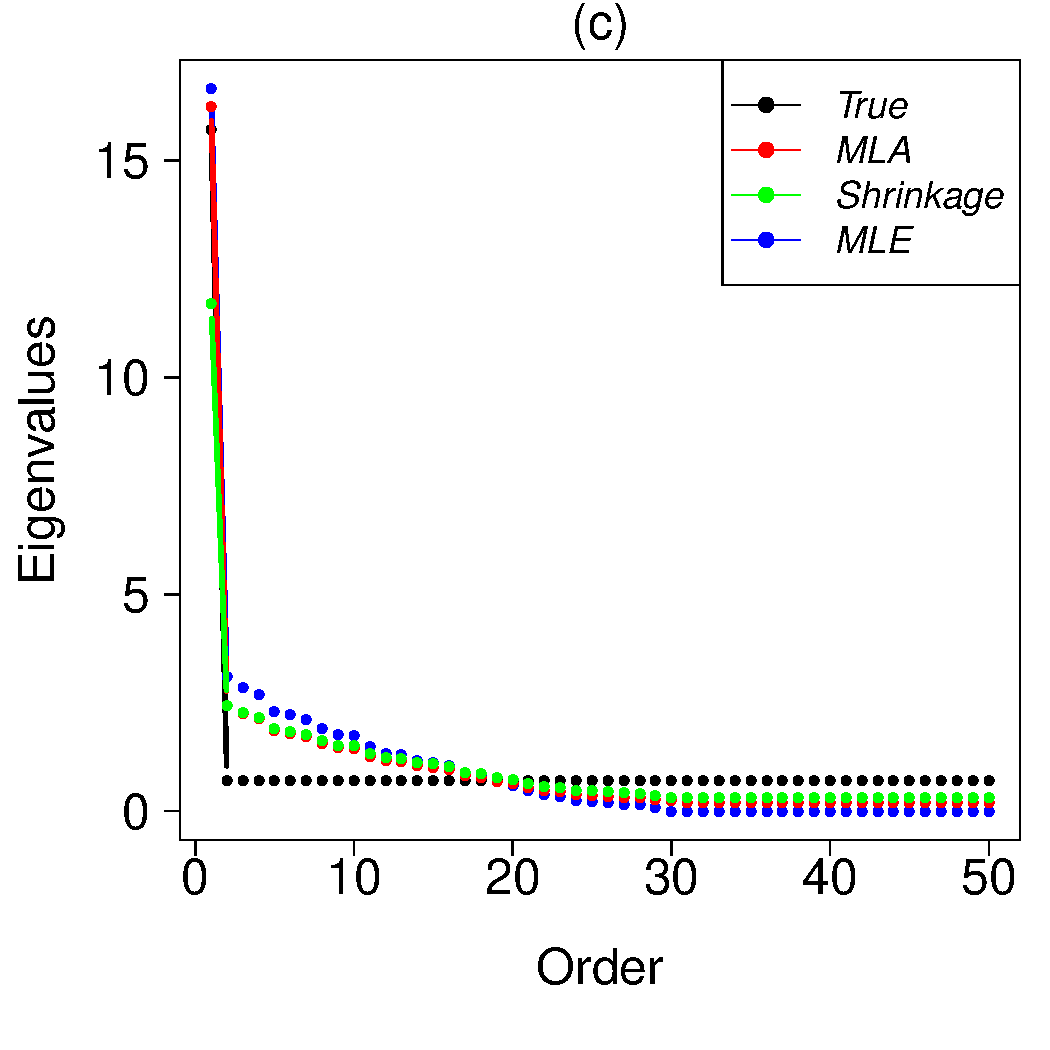
\includegraphics[scale=0.33]{FIG4_3c.pdf}
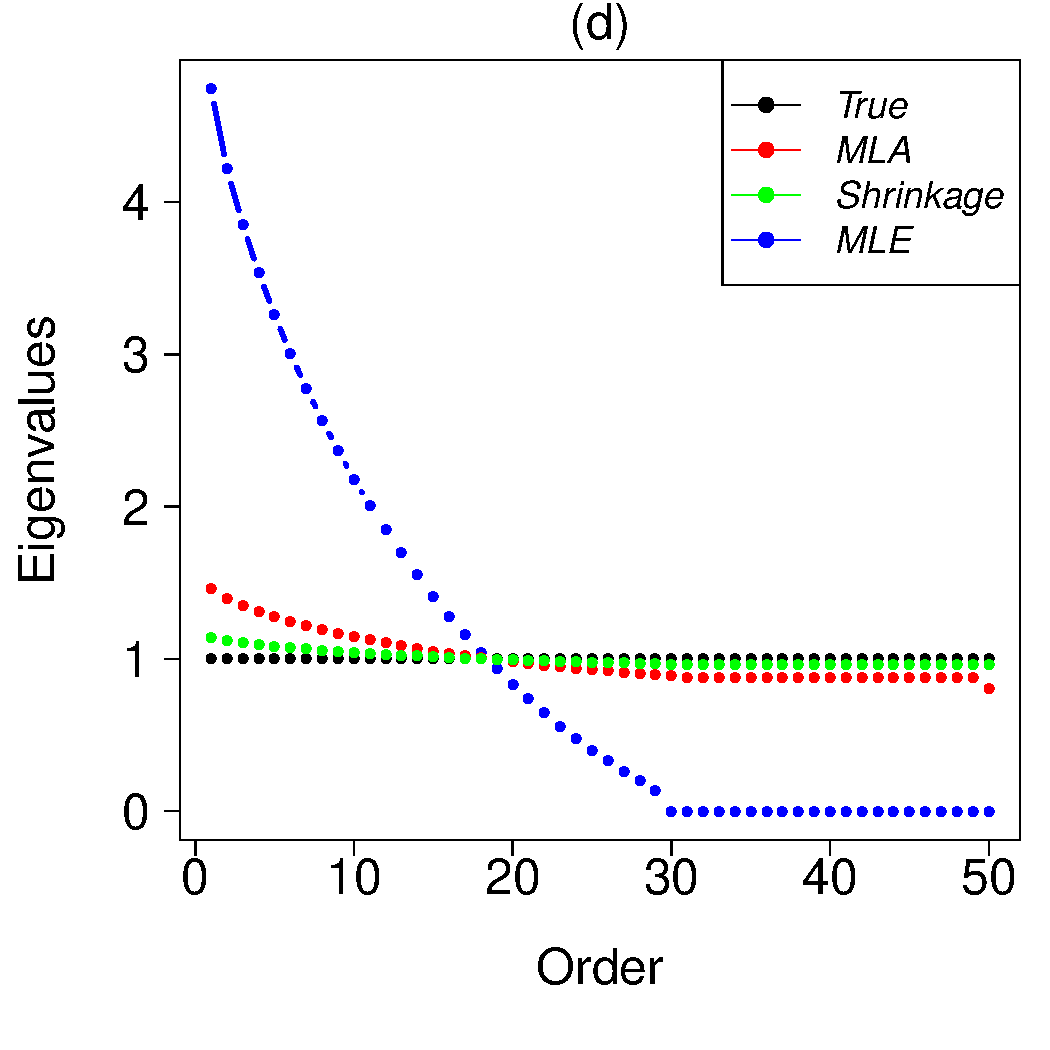
\includegraphics[scale=0.33]{FIG4_3d.pdf}
\end{array}$
\end{center}
\begin{center}$
\begin{array}{r}
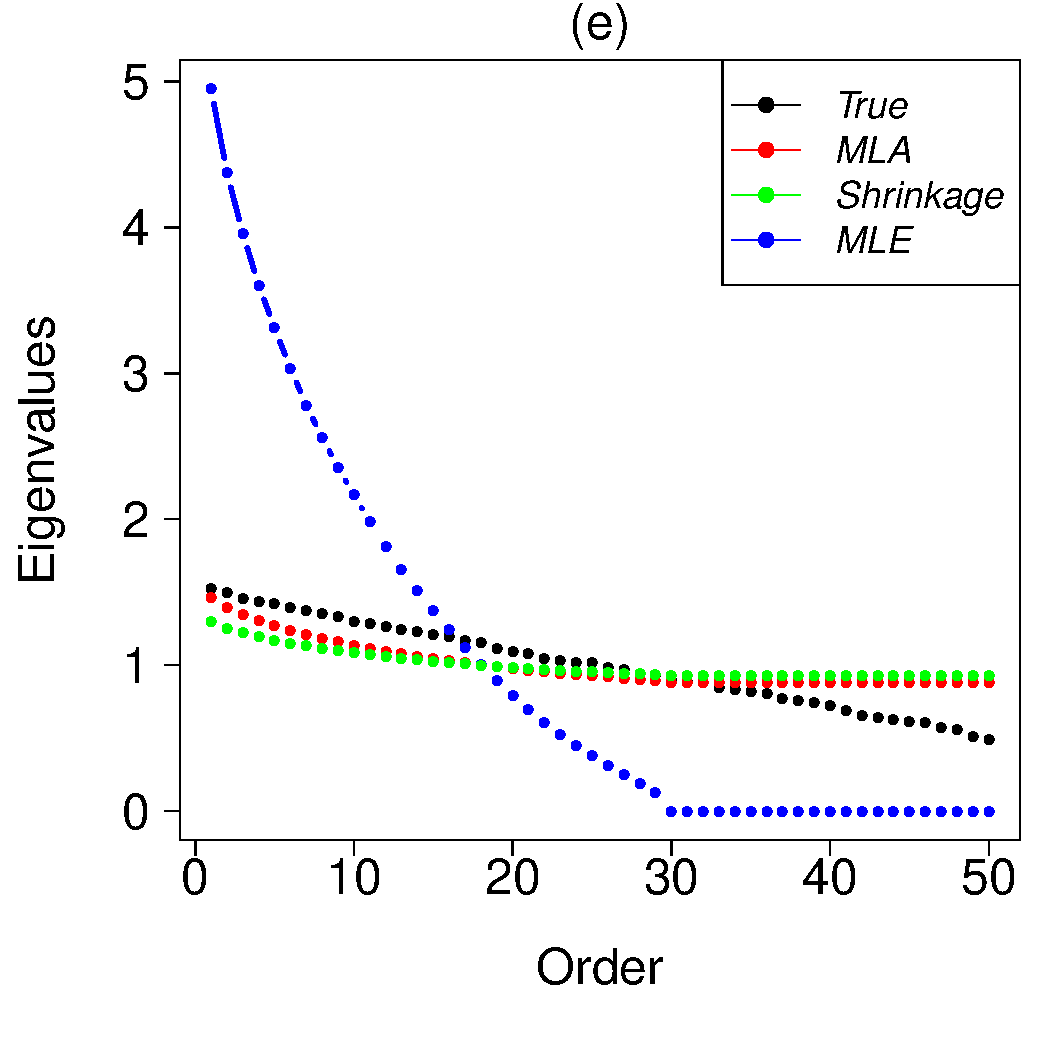
\includegraphics[scale=0.33]{FIG4_3e.pdf}
\end{array}$
\end{center}
\caption{Comparison of estimated and true eigenvalues with $n=30$ and $p=50$ averaged over 1000 simulation. The data are drawn from multivariate normal distribution under different choices of covariance matrices (a, b) AR(1) with $t=0.5$ and identity as true covariance matrix for all three methods and AR(1) as a target for the proposed method (c, d) exchangeable with $t=0.3$ and identity as true covariance matrix for all three methods and exchangeable as a target for the proposed method (e) random covariance structure with 30\% off-diagonal entries as non-zero and identity matrix as a target.}
\label{Fig3}
\end{figure}


%\begin{figure}[h]
%\centering
%\begin{subfigure}[t]{.4\textwidth}
%\centering
%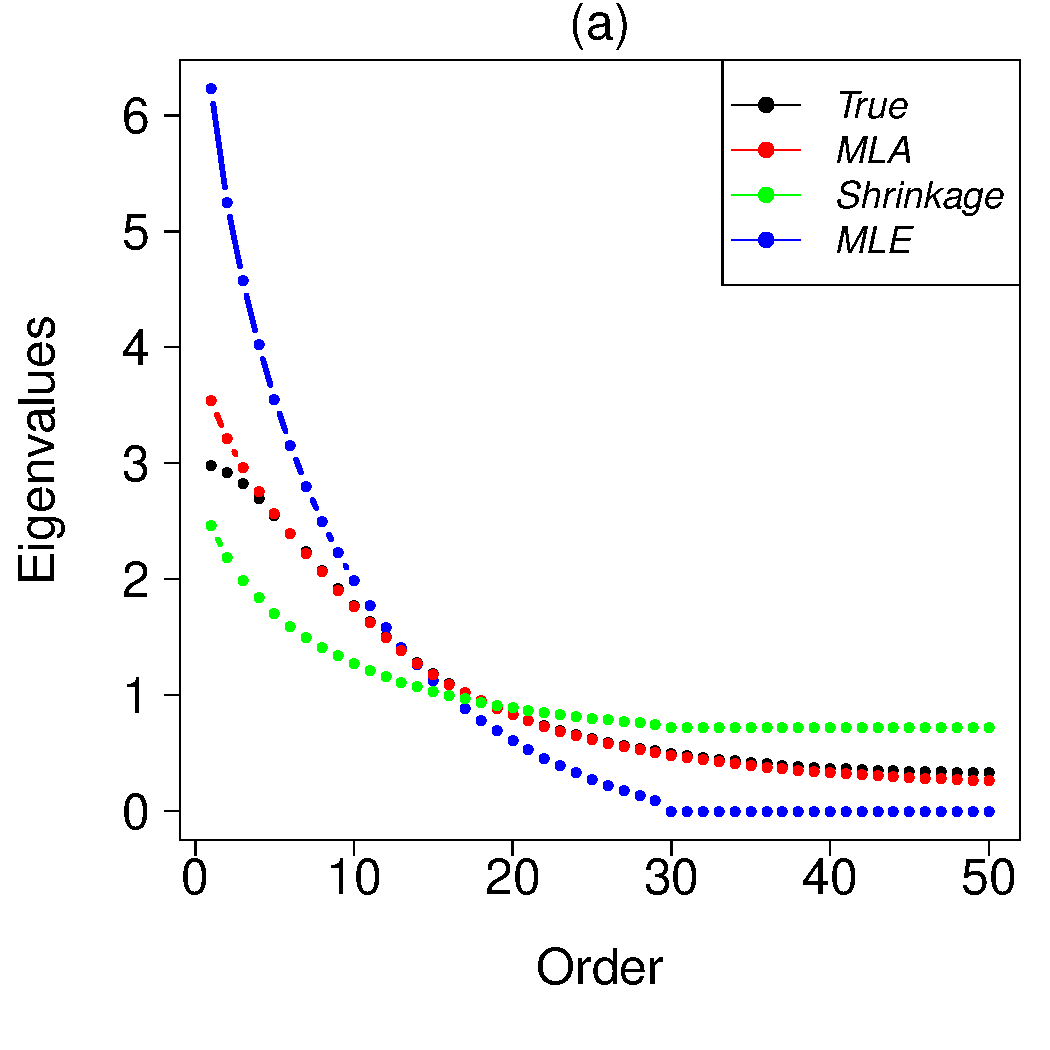
\includegraphics[width=\linewidth]{FIG4_3a.pdf}
%\end{subfigure}
%\begin{subfigure}[t]{.4\textwidth}
%\centering
%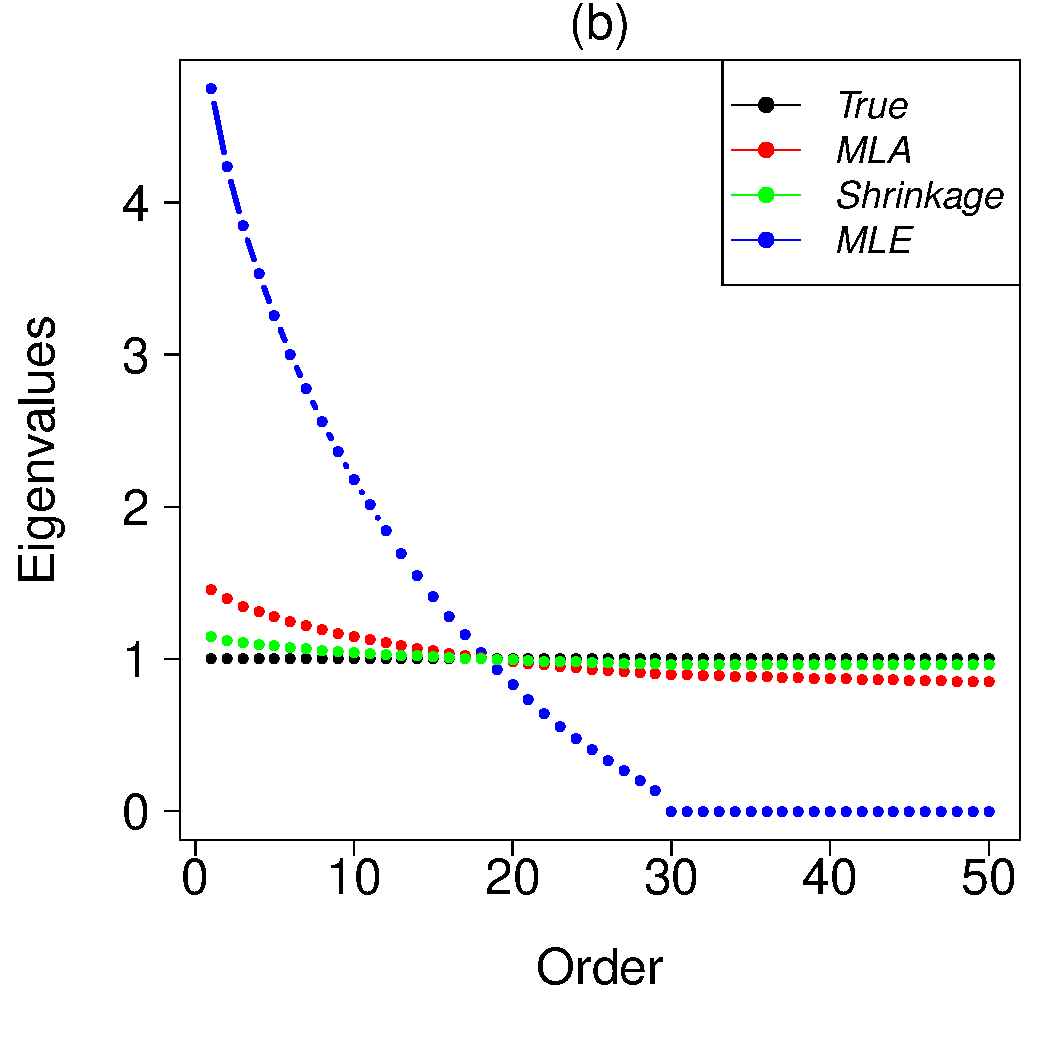
\includegraphics[width=\linewidth]{FIG4_3b.pdf}
%\end{subfigure}
%\medskip
%\begin{subfigure}[t]{.4\textwidth}
%\centering
%\vspace{0pt}
%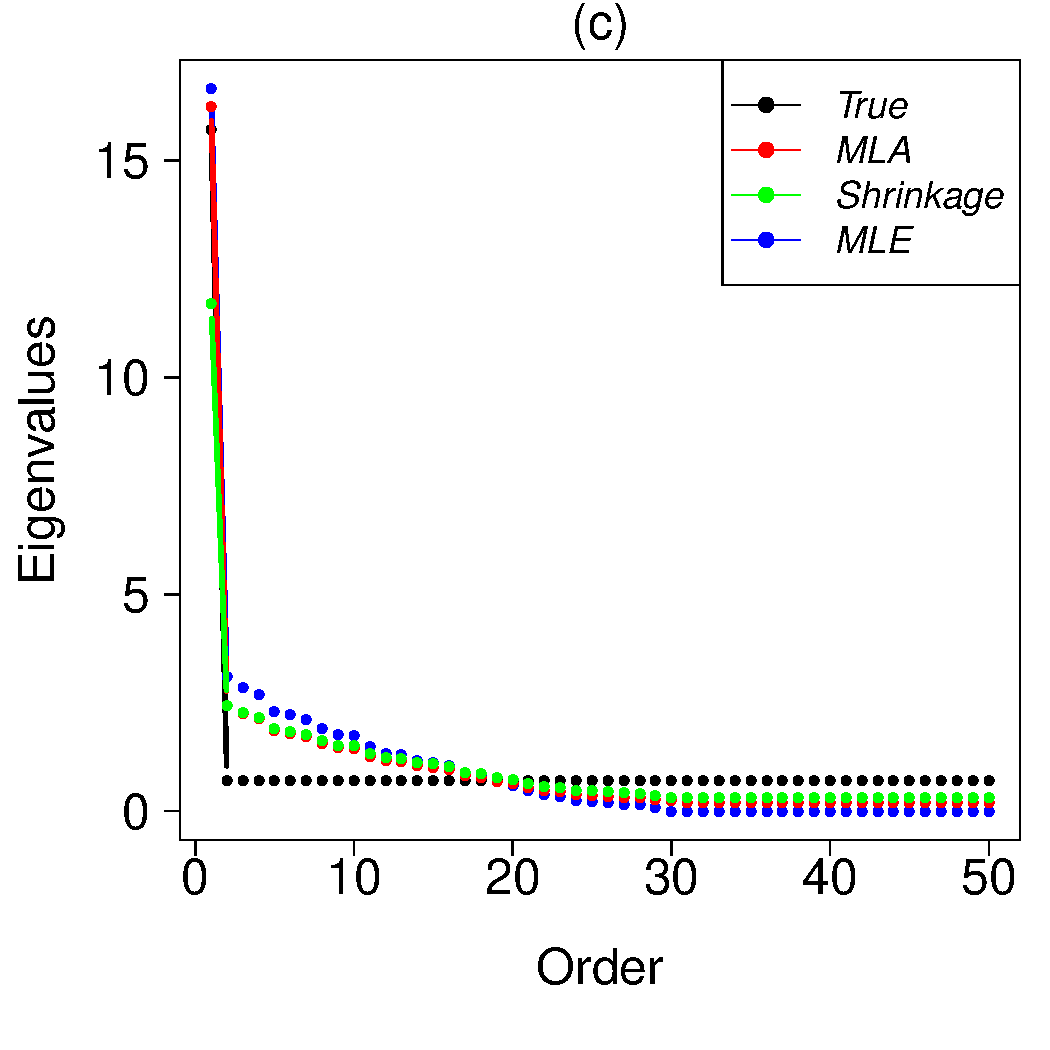
\includegraphics[width=\linewidth]{FIG4_3c.pdf}
%\end{subfigure}
%\begin{subfigure}[t]{.4\textwidth}
%\centering
%\vspace{0pt}
%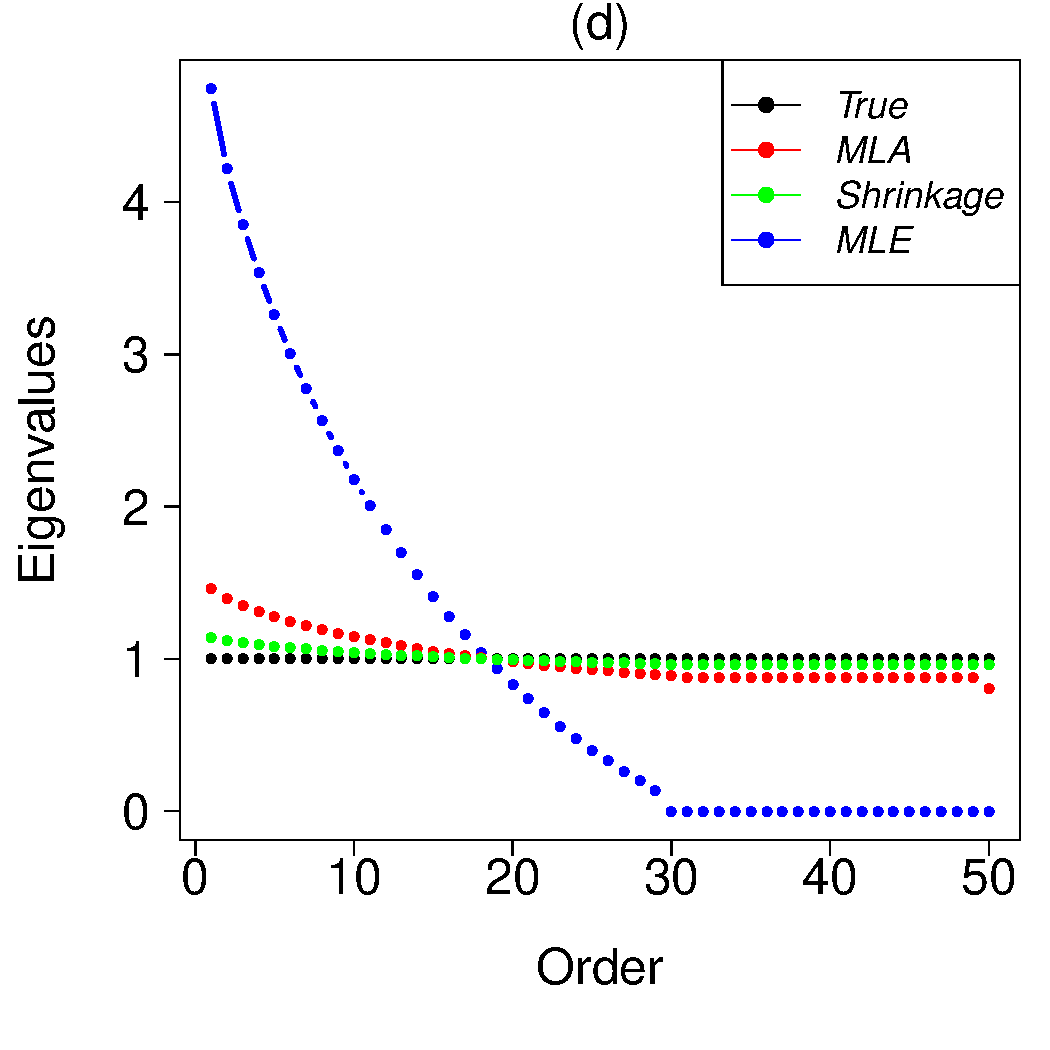
\includegraphics[width=\linewidth]{FIG4_3d.pdf}
%\end{subfigure}
%\begin{subfigure}[t]{.4\textwidth}
%\centering
%\vspace{0pt}
%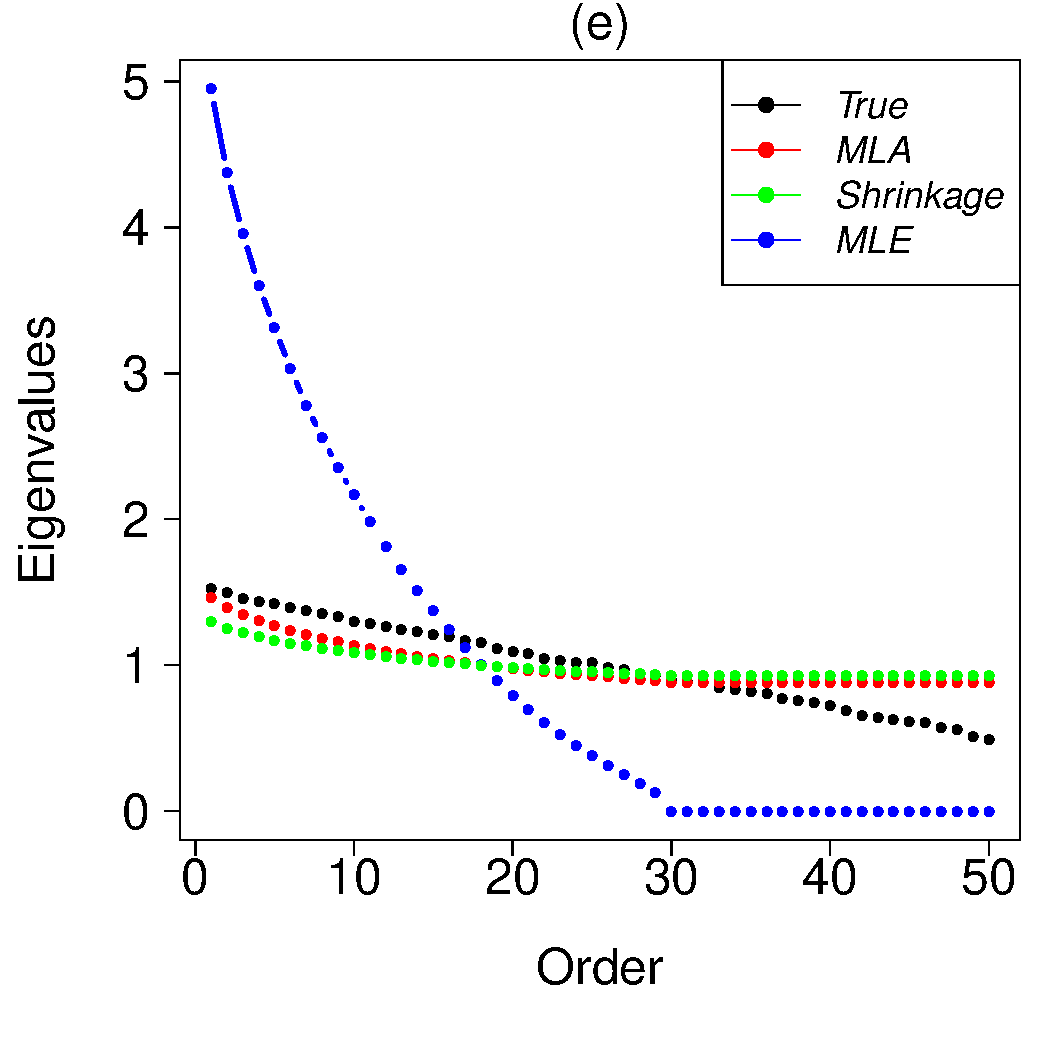
\includegraphics[width=\linewidth]{FIG4_3e.pdf}
%\end{subfigure}
%\caption{Comparison of the estimated and true eigenvalues with $n=30$ and $p=50$ averaged over 1000 simulation. The data are drawn from multivariate normal distribution under different covariance structures arranged in Table \ref{Tab1} with different targets for the proposed method. For random covariance structure we took 30\% off-diagonal entries as being non-zero.}
%\label{Fig3}
%\end{figure}
